\documentclass[11pt]{article}

% Korean academic article preamble -- XeLaTeX
\usepackage{kotex}
\usepackage{fontspec}
\usepackage{unicode-math}
\usepackage{mathtools,amssymb,amsthm}
\usepackage{booktabs,threeparttable,array}
\usepackage{graphicx}
\usepackage{xcolor}
\usepackage{setspace}
\usepackage{enumitem}
\usepackage{microtype}
\usepackage{titlesec}
\usepackage[
  a4paper,
  top=25mm,
  bottom=25mm,
  left=28mm,
  right=28mm
]{geometry}

\defaultfontfeatures{Ligatures=TeX}
\IfFontExistsTF{STIX Two Text}{
  \setmainfont{STIX Two Text}
}{
  \setmainfont{TeX Gyre Termes}
}
\IfFontExistsTF{STIX Two Math}{
  \setmathfont{STIX Two Math}
}{
  \setmathfont{Latin Modern Math}
}
\IfFontExistsTF{KoPubWorld Batang Pro}{
  \setmainhangulfont{KoPubWorld Batang Pro}
  \setsanshangulfont{KoPubWorld Dotum Pro}
}{
  \IfFontExistsTF{Noto Serif CJK KR}{
    \setmainhangulfont{Noto Serif CJK KR}
    \setsanshangulfont{Noto Sans CJK KR}
  }{}
}

\definecolor{LinkBlue}{HTML}{2457A6}
\definecolor{MutedGray}{HTML}{5F6368}

\usepackage[round,authoryear]{natbib}
\usepackage{hyperref}
\hypersetup{
  unicode=true,
  colorlinks=true,
  linkcolor=LinkBlue,
  citecolor=LinkBlue,
  urlcolor=LinkBlue,
  pdftitle={복권식 경마시장의 정보 집계},
  pdfauthor={김주철}
}

\setstretch{1.38}
\setlength{\parindent}{1em}
\setlength{\parskip}{0pt}
\setlist{nosep,leftmargin=2em}
\emergencystretch=2em

\titleformat{\section}
  {\large\sffamily\bfseries}{\thesection.}{0.65em}{}
\titleformat{\subsection}
  {\normalsize\sffamily\bfseries}{\thesubsection.}{0.65em}{}
\titlespacing*{\section}{0pt}{2.8ex plus 0.6ex minus 0.3ex}{1.1ex}
\titlespacing*{\subsection}{0pt}{2.2ex plus 0.5ex minus 0.2ex}{0.8ex}

\newtheorem{proposition}{명제}
\newcommand{\E}{\mathbb{E}}
\newcommand{\R}{\mathbb{R}}
\newcommand{\one}{\mathbf{1}}
\newcommand{\T}{\mathsf{T}}
\newcommand{\W}{\mathsf{W}}
\newcommand{\Eact}{\mathsf{E}}
\newcommand{\Q}{\mathsf{Q}}
\newcommand{\Trio}{\mathsf{R}}

\renewcommand{\abstractname}{초록}
\renewcommand{\refname}{참고문헌}
\renewcommand{\tablename}{표}
\renewcommand{\figurename}{그림}


\title{\textbf{경마 베팅시장의 정보 집계}\\
  \large 삼쌍승식 상태가격의 교차풀 정합성과 3단계 행동모형}
\author{김주철\\\small 연세대학교}
\date{}

\begin{document}

\maketitle

\begin{abstract}
하나의 경주에서는 같은 결과를 서로 다르게 분할한 단승식, 복승식, 쌍승식,
삼복승식과 삼쌍승식 청구권이 별도 패리뮤추얼 풀에서 거래된다. 이 논문은
2016년 6월부터 2025년 12월까지 한국마사회 19,284개 경주를 이용하여, 이
복수 가격이 하나의 상위 3위 상태공간과 얼마나 정합적인지, 남은 가격차가
복합복권의 축약과 순차평가 중 어느 표현과 더 잘 양립하는지 두 층으로
검정한다.

첫째, 삼쌍승식 순위별 역배당률로 완전한 1--3위 정규화 가격분포를 구성하고
이를 주변화하여 다른 승식의 가격을 재구성한다. 배당상한이 없는 3,321개
clean 경주의 점추정과 전체 19,284개 경주의 검열·반올림 부분식별 경계를
공동 주결과로 사용한다. 삼쌍승 주변가격은 쌍승·복승·삼복승에서 단승 기반
Harville뿐 아니라 순열·타경주·균등 기준보다 일관되게 실제 가격에 가깝고,
이 우위는 전체표본의 보수적 부분식별에서도 유지된다. 그러나 사전에 정한
절대 TV 기준을 두 패널이 동시에 통과하지 못하므로, 결과는 완전한 공통
상태가격이 아니라 높지만 불완전한 교차풀 가격 정합성을 뜻한다.

둘째, 연도 밖 착순으로 조건부 순위확률을 추정하고 단승 가격에서 고정한
가중함수를 다른 승식의 전체 가격벡터에 적용한다. 결합사건에 가중함수를 한 번
적용하는 축약모형보다 조건부 순위를 단계별로 평가하는 모형의 가격오차가
쌍승·삼쌍승에서 작고, 다시 맞추지 않은 복승·삼복승 외부검증에서도 같은
순위가 유지된다. 3단계 모형의 삼복승 TV 중앙값은 0.1545다. 이 결과는
복합복권 비축약과 양립하지만, 위험선호와 확률오인을 개별적으로 식별하거나
개인의 인지과정을 직접 관찰한 것으로 해석하지 않는다.

\medskip
\noindent\textbf{핵심어:} 경마시장, 교차풀 정합성, 상태가격, 삼쌍승식,
확률가중, 복합복권
\end{abstract}

\begin{center}
\small
\textbf{Information Aggregation Across Parimutuel Wagering Markets:}
Cross-Pool Coherence and Three-Stage Behavioral Models from Trifecta Prices
\end{center}

\section{서론}

한 경주의 단승식, 복승식, 쌍승식, 삼복승식과 삼쌍승식은 같은 실현결과에
연동되지만 서로 다른 사건에 지급하고 별도 패리뮤추얼 풀에서 청산된다. 따라서
각 풀의 마감 배당률은 동일한 기초 순위에 대한 서로 다른 가격측도를 제공한다.
이 구조는 두 질문을 낳는다. 여러 풀의 전체 가격벡터는 하나의 상위 3위
상태공간에서 나온 주변분포와 얼마나 가까운가? 그 정합성에서 벗어난 가격차를
복합복권의 행동모형이 강화된 순위 기준모형보다 더 잘 설명하는가?

기존 경마시장 연구는 주로 단승 배당률이 시사하는 확률과 사후 승률을 비교하여
인기마--비인기마 편향을 검정했다. 비인기마가 과대 베팅되고 인기마가 과소
베팅된다는 결과는 오래된 경험적 규칙성이지만
\citep{griffith1949,weitzman1965,ali1977}, 홍콩처럼 편향이 약하거나 반대로
나타난 시장도 있다 \citep{buschehall1988}. 한국 자료에서는 말과 경주의
이질성을 허용한 승률모형으로 전형적 편향이 보고됐고
\citep{jeongetal2019}, 게시 배당률의 반올림 자체가 전통적 검정통계를
왜곡할 수 있다는 지적도 있다 \citep{wallsbusche2003}. 이 문헌은 위험선호,
확률 오인, 참가자 이질성과 측정오차를 구분해 왔지만, 한 시장의 배당률과
실현결과만으로는 위험선호와 확률오인이 같은 가격패턴을 만들 수 있다.

\citet{snowbergwolfers2010}는 단승식에서 추정한 두 설명이 쌍승·복승·삼쌍승
가격으로 이동하는지를 비교하여 이 관측적 동등성에 제약을 가했다. 다만 이들의
자료에는 exotic 승식의 당첨 배당만 있고 비당첨 조합의 가격은 없었다.
\citet{koivurantakorhonen2019}은 핀란드와 스웨덴의 완전한 exotic 가격을
이용하여 당첨조합 선택 문제를 줄이고, 1위와 2위를 순차적으로 평가하는 모형을
검정했다. 따라서 완전한 복합승식 가격 자체는 새로운 기여가 아니다. 남은
질문은 순서 있는 상위 3위 전체 상태를 여러 하위 승식과 동시에 연결할 때,
교차풀 가격 정합성과 세 번째 조건부 평가단계를 무엇까지 식별할 수 있는가이다.

이 논문은 연구를 두 층으로 나눈다. 첫째 층인 주분석에서는 삼쌍승식의 각
조합을 ``1위 $i$, 2위 $j$, 3위 $k$''라는 원자적 상태로 해석한다. 삼쌍승식
역배당률을 경주 안에서 정규화한 뒤 합산하면 단승, 쌍승, 복승, 삼복승이
지급하는 사건의 재구성 가격을 얻는다. 이 가격을 각 승식의 실제 정규화 가격과
비교하여 객관적 승률을 추정하지 않고도 교차풀 정합성을 측정한다.

게시 표시상한은 이 비교의 부차적 문제가 아니다. 상한 없는 경주의 점추정은
정확하지만 표본선택에 노출되고, 상한 경주를 포함한 전체표본은 가격을 구간으로만
식별한다. 따라서 이 논문은 clean 표본의 점추정과 전체표본의 부분식별 경계를
공동 주결과로 두고, 두 결과가 같은 방향을 지지할 때만 전체 시장에 관한 강한
결론을 허용한다.

둘째 층은 Snowberg and Wolfers의 검정논리를 세 번째 순위까지 확장하되,
실현 착순으로 조건부 순위확률을 표본 밖에서 추정한 뒤, 단승 가격에 맞춘
확률가중 함수가 다른 풀의 전체 가격벡터를 설명하는지 검정한다.
특히 삼쌍승 사건의 결합확률에 확률가중을 한 번 적용하는 축약 모형,
`1위→나머지 두 순위`의 2단계 모형, `1위→2위→3위`의 3단계 비축약 모형을
비교한다. 순서가 없는 승식에는 임의의 사건트리를 부여하지 않고, 순서형 모형의
풀 밖 예측을 검증하는 데 사용한다. 동시에 게시가격 Harville(비보정)과 연도 밖
착순으로 추정한 보정·단계조정 Harville을 같은 경주에 적용하여 행동모형의 추가 설명력을
직접 비교한다.

결과는 두 층의 구분이 실제로 중요함을 보여준다. 주분석에서 삼쌍승 주변가격은
하위 복합승식을 Harville과 비정보적 기준보다 일관되게 잘 재구성하지만,
사전에 정한 강한 절대 TV 기준은 clean 점표본과 전체표본 경계를 동시에
통과하지 못한다. 진단분석에서 보정·단계조정 조건부 순위확률은 보정 Harville($\alpha=1$)보다
2·3위의 연도 밖 로그손실과 보정오차를 낮춘다. M-S2/M-S3은 M-R보다
가격오차가 작지만, 동일표본의 단계조정 Harville을 네 승식 어디에서도 넘지
못한다. 이 판정은 공통지지 조합과 최저가격 10\%를 제외한 조합에서도 유지된다.
따라서 가격의 교차풀 정합성은 높지만 완전하지 않으며, 그 잔여 차이를 비축약
행동으로 구조적으로 해석할 증거는 얻지 못한다.

이 연구의 기여는 세 가지다. 첫째, 완전한 삼쌍승 가격벡터와 고정된 주변화
행렬을 이용하여 다섯 풀의 가격을 하나의 상위 3위 상태공간에서 비교한다.
둘째, Harville·동일 경주 순열·타경주·균등 기준을 같은 표본과 손실함수에서
비교하고, 점추정과 전체표본 부분식별 경계를 나란히 두어 높은 적합도가 공통
인기순위·차원 또는 선택된 clean 표본의 산물인지 구분한다. 셋째,
복합복권의 축약 여부를 세 번째 순위까지 확장하되 게시가격 Harville(비보정)과
보정·단계조정 Harville을
동일표본 기준으로 함께 두어, 내부적인 M-R 대비 개선과 독립적인 행동설명력을
구분한다.

여기서 ``재구성력이 높다''는 말은 삼쌍승식 가격이 객관적 확률이라는 뜻이
아니다. 별도 풀의 정규화 역배당률을 같은 가격측도의 주변분포로 해석하려면
정보시점, 공제·반올림, 참가자 구성과 평가기능에 관한 유지가정이 필요하다.
그 가정을 유지하지 않으면 주분석은 서로 다른 풀 가격측도의 정적 정렬 정도를
측정한다. 또한 M-S의 M-R 대비 우위는 집계가격의 내부 모형순위일 뿐이며,
더 강한 비행동 기준모형을 이기지 못한 이상 개별 베팅자의 심리과정에 대한
증거가 아니다. 본문은 이 두 해석의 경계를 분리한다.

\section{제도와 관련 문헌}

\subsection{한국 경마의 복수 패리뮤추얼 시장}

패리뮤추얼 시장에서는 같은 조합에 걸린 금액이 하나의 풀을 이루고, 공제 후
풀이 적중권에 배분된다. 따라서 게시 배당률은 고정된 북메이커 가격이 아니라
마감 시점의 상대 베팅액을 반영한다. 각 승식은 별도의 풀을 가지므로 공제율,
유동성, 참가자 구성, 배당률 절사 방식의 차이가 교차시장 가격 차이로 남을 수
있다.

\begin{table}[htbp]
\centering
\caption{상위 3위 상태와 주요 승식의 지급 사건}
\label{tab:market-events}
\begin{tabular}{lll}
\toprule
승식 & 지급 사건 & 삼쌍승 상태의 합산 범위 \\
\midrule
단승식 & $i$가 1위 & 고정 $i$, 모든 $j,k$ \\
쌍승식 & $i$가 1위, $j$가 2위 & 고정 $i,j$, 모든 $k$ \\
복승식 & $i,j$가 순서 없이 1·2위 & 고정 $\{i,j\}$, 모든 $k$ \\
삼복승식 & $i,j,k$가 순서 없이 1--3위 & 여섯 순열 \\
삼쌍승식 & $i,j,k$가 정확히 1·2·3위 & 하나의 $(i,j,k)$ \\
\bottomrule
\end{tabular}
\end{table}

연승식과 복연승식은 출전두수에 따라 적중 순위의 범위가 달라질 수 있으므로
주 분석의 단순 주변화 대상에서 제외하고, 공식 승식 규칙을 적용한 별도
강건성 분석으로 다룬다. 이 구분은 편의가 아니라 지급 사건을 정확히 일치시키기
위한 사전 규칙이다.

\subsection{인기마--비인기마 편향과 정보 집계}

\citet{griffith1949}, \citet{weitzman1965}, \citet{ali1977}는 배당률이
시사하는 확률과 실제 승률의 체계적인 차이를 기록했다. 이후 연구는 이 패턴을
위험애호로 읽을 것인지, 낮은 확률의 과대평가로 읽을 것인지 논쟁해 왔다.
\citet{julliensalanie2000}은 위험 아래 선호를 구조적으로 추정했고,
\citet{snowbergwolfers2010}는 위험선호와 확률 오인 설명을 식별하는 검정을
제시했다. \citet{coleman2004}은 여러 국가의 결과를 종합하여 서로 다른 정보와
위험태도를 가진 참가자 집단의 혼합을 한 설명으로 제안했고,
\citet{suhonenetal2018}은 이중이론과 확률가중을 결합하여 패리뮤추얼 자료의
선택을 설명한다.

시장의 차이도 중요하다. \citet{buschehall1988}은 홍콩 시장에서 전형적
편향의 예외를 보고했고, \citet{vaughanwilliams1997}과
\citet{vaughanwilliams1998}은 정보비용, 소비효용, 참가자 이질성이 시장별
편향의 부호를 바꿀 수 있음을 논의한다. \citet{brucejohnson2000}은 병행하는
북메이커와 패리뮤추얼 시장을 비교했고, \citet{sungjohnsonpeirson2012}은
정보가 부족한 참가자의 비중이 가격오류에 미치는 영향을 분석했다.
\citet{shin1991}은 내부정보 거래자가 존재하는 북메이커 모형에서 게시가격이
승률과 체계적으로 벌어질 수 있음을 보였다. 이는 패리뮤추얼 시장을 직접
모형화한 결과는 아니지만, 정보 비대칭이 가격과 기초확률의 괴리를 낳을 수
있는 한 경로를 제시한다.

한국어 문헌도 국내 시장의 서로 다른 측면을 분석했다.
유웅·남준우\citeyearpar{yoonam2015}는 수익률의
평균과 분산에 왜도를 더한 효용함수를 추정하여, 비인기마 선택을 위험애호만으로
해석하기보다 위험회피와 양의 왜도 선호가 함께 나타날 수 있음을 보였다.
같은 저자들\citeyearpar{yoonam2017}은 국내 복승식 자료에서 비선호마 편향과
베팅 전략의 수익률을 분석하여 가격 효율성의 문제를 제기했다.
최혜민 외\citeyearpar{choietal2015}는 경주마·기수·조교사 정보를 사용한 우승마
예측모형을 구축하고, 단승식·복승식·삼복승식의 표본 외 베팅 결과를 비교했다.
이 연구들은 각각 베팅자의 선호, 특정 승식의 가격 효율성, 실현 착순에 대한
외부 예측력을 다룬다.

한국 시장에 대해서는 \citet{jeongetal2019}가 말과 경주의 이질성을 허용하는
승률 모형으로 인기마--비인기마 편향을 검정했다. 본 논문은 이들 연구를 대체하지
않는다. 실현 승률을 추정하거나 개별 승식의 투자수익률을 평가하는 대신, 동일
경주의 복수 승식 가격이 하나의 순위 상태분포에서 나올 수 있는지 검정한다는
점에서 질문과 식별 대상이 다르다.
또한 게시 배당률의 반올림은 인기마 구간의 검정통계에 체계적인 영향을 줄 수
있으므로 \citep{wallsbusche2003}, 원자료의 배당 단위와 상한을 명시적으로
점검한다.

\section{주분석: 가격측도와 교차풀 제약}

\subsection{게시가격과 삼쌍승식 상태분포}

경주 $r$의 유효 출전마 집합을 $N_r$, 유효 출전마 수를 $n_r=|N_r|$라 하고,
순서 있는 상위 3마리의 상태공간을
\[
  \Omega_r=\{(i,j,k)\in N_r^3:i,j,k\text{는 서로 다르다}\}
\]
로 둔다. 삼쌍승식 상태 $(i,j,k)$의 게시 총지급배율을 $D^{\T}_{r,ijk}$라 하자.
KRA 배당률은 원금을 포함하므로 단위지급 청구권의 게시가격은
$x^{\T}_{r,ijk}=1/D^{\T}_{r,ijk}$다. 순수익 배당을 $O/1$로 표시하는 문헌의
가격 $1/(O+1)$과 같은 개념이지만, 표기법은 구분한다.

주분석에서는 역배당률을 경주와 풀 안에서 정규화한
\begin{equation}
  q^{\T}_{r,ijk}
  =\frac{x^{\T}_{r,ijk}}
  {\sum_{(a,b,c)\in\Omega_r}x^{\T}_{r,abc}}
  \label{eq:trifecta-state-price}
\end{equation}
을 삼쌍승식 정규화 가격측도라 부른다. 이상적인 패리뮤추얼 풀에서 이는 풀의
조합별 베팅금액 비중과 대응한다. 객관적 순위확률이나 Arrow--Debreu 상태가격을
복원한다고 전제하지 않는다. 정규화는 풀 전체에 공통으로 곱해지는 공제 요인을
제거하지만 조합별 반올림, 유동성 차이와 마감 직전 베팅의 영향은 제거하지 않는다.

\subsection{주변화 연산}

삼쌍승식 분포가 주어지면 단승식, 쌍승식, 복승식의 재구성 가격은 각각
\begin{align}
  \widehat p^{\W\leftarrow\T}_{r,i}
    &=\sum_{j\ne i}\sum_{k\notin\{i,j\}}q^{\T}_{r,ijk},
    \label{eq:win-marginal}\\
  \widehat p^{\Eact\leftarrow\T}_{r,ij}
    &=\sum_{k\notin\{i,j\}}q^{\T}_{r,ijk},
    \label{eq:exacta-marginal}\\
  \widehat p^{\Q\leftarrow\T}_{r,\{i,j\}}
    &=\sum_{k\notin\{i,j\}}
      \left(q^{\T}_{r,ijk}+q^{\T}_{r,jik}\right)
    \label{eq:quinella-marginal}
\end{align}
이다. 삼복승식은 세 말의 여섯 순열을 합한다.
\begin{equation}
  \widehat p^{\Trio\leftarrow\T}_{r,\{i,j,k\}}
  =\sum_{\pi\in S_3}q^{\T}_{r,\pi(i,j,k)}.
  \label{eq:trio-marginal}
\end{equation}

각 하위 승식 $m$의 게시가격도 같은 방식으로 정규화하여 $p^m_r$를 만든다.
$A^m_r$를 식 \eqref{eq:win-marginal}--\eqref{eq:trio-marginal}의 합산을 나타내는
0--1 incidence matrix라 하면 완전한 교차풀 제약은
\begin{equation}
  p^m_r=A^m_r q^{\T}_r
  \label{eq:cross-market-restriction}
\end{equation}
이다. 실제 분석은 등식의 성립을 전제하지 않고 좌우의 거리를 측정한다.

\subsection{공통 가격측도 해석의 유지가정}

식 \eqref{eq:cross-market-restriction}을 하나의 공통 가격측도에서 나온 주변분포로
해석하려면 네 가지 유지가정이 필요하다. 첫째, 각 풀의 최종 가격이 같은
정보시점을 반영하고 취소마와 지급사건의 정의가 일치해야 한다. 둘째, 공제율은
풀 안에서 공통 배율로 작용하고 반올림·절사·적중자 없음 규칙이 조합별
상대가격을 크게 바꾸지 않아야 한다. 셋째, 별도 풀의 참가자 구성과 대표적
신념·평가기능이 같거나 안정적으로 연결되어야 한다. 넷째, 유동성과 최소
베팅단위가 풀별 비선형 왜곡을 만들지 않아야 한다.

이 가정이 모두 성립하지 않아도 주변화 연산 자체는 정확하다. 다만 이때 거리는
서로 다른 풀 가격측도의 \emph{정적 정렬 정도}이며, 무차익 상태가격의 존재나
개별 참가자의 합리성을 검정하지 않는다. 이 구분 때문에 본 논문은
``공통 상태가격을 입증한다''보다 ``공통 가격측도와의 양립 정도를 측정한다''고
표현한다.

\subsection{Harville 기준모형}

단승식 정규화 가격 $p^{\W}_{r,i}$만을 이용하는 Harville형 순차
모형\citep{harville1973}은
\begin{equation}
  q^{H}_{r,ijk}
  =p^{\W}_{r,i}
   \frac{p^{\W}_{r,j}}{1-p^{\W}_{r,i}}
   \frac{p^{\W}_{r,k}}{1-p^{\W}_{r,i}-p^{\W}_{r,j}}
  \label{eq:harville}
\end{equation}
로 정의한다. 이는 한 말이 먼저 들어온 뒤 남은 말의 상대확률이 비례적으로
재조정된다는 강한 가정을 둔다. 삼쌍승식 가격측도의 주변분포가
$A^m_rq^H_r$보다 실제 쌍승·복승·삼복승 가격에 더 가깝다면, 그 차이를
삼쌍승식 가격이 담은 순위 의존 구조의 증분으로 해석한다. 두 모형 모두
시장가격에서 출발하므로 이는 인과적 정보효과가 아니라 가격 설명력의 차이다.

\section{자료와 표본}

자료는 한국마사회 공개 경주자료에서 수집한 승식별 최종 배당률이다. 삼쌍승식이
도입된 2016년 6월 10일부터 2025년 12월 31일까지를 기본 범위로 한다. 코로나19
기간의 시장 운영이 평시와 크게 달랐던 2020년과 2021년은 제외한다. 이 범위의
파싱된 후보 자료는 2016--2019년과 2022--2025년의 19,301개 경주다. 원자료에
9,999를 넘는 값이 확인된 2018년 7월 1일의 17개 경주를 사전 규칙에 따라
제외하면 19,284개 경주가 남는다. 최종 분석표본과 조건별 제외 경주 수는 재현
스크립트가 생성한 \texttt{outputs/sample\_flow.csv}에서 확인할 수 있다.

분석 단위는 경주--승식--조합이다. 각 경주에서 유효 출전마 목록을 먼저 고정한
뒤, 이 목록으로 가능한 조합의 완전한 지지집합을 생성한다. 취소마, 판매중지
조합, 중복 레코드, 0 이하이거나 유한하지 않은 배당률을 순서대로 처리한다.
삼쌍승식의 관측 조합 수가 $n_r(n_r-1)(n_r-2)$와 일치하지 않는 경주는 결측
원인을 기록하고 주 분석에서 제외한다. 단순히 존재하는 행만 다시 정규화하면
결측 상태의 질량을 나머지 상태에 잘못 배분할 수 있기 때문이다.

주분석은 완전한 가격 지지집합을 요구하지만 행동모형에는 실현 착순도 필요하다.
행동모형 표본에서는 1--3위 착순과 유효 출전마의 대응을 추가로 검증한다.
조건부 순위확률을 추정하는 자료와 구조모형의 가격예측을 평가하는 자료는 연도를
fold로 나누어 교차적합한다. 따라서 같은 경주의 실현 착순으로 그 경주의
객관확률을 추정한 뒤 같은 가격에 맞추는 순환을 허용하지 않는다.

자료 검증은 다음 네 층으로 나눈다.

\begin{enumerate}
  \item \textbf{키 검증}: 날짜, 경마장, 경주번호, 승식, 조합이 유일한지 확인한다.
  \item \textbf{지지집합 검증}: 유효 출전마와 승식별 가능한 조합이 일치하는지 확인한다.
  \item \textbf{가격 검증}: 배당률의 단위, 최솟값, 게시 상한과 소수 첫째 자리 표기 구조를 확인한다.
  \item \textbf{재현 검증}: 원자료 파싱부터 논문의 표·그림까지 하나의 명령으로 다시 만든다.
\end{enumerate}

감사 결과, 사전 날짜 규칙을 통과한 19,284개 경주에서는 단승·쌍승·복승·
삼복승·삼쌍승 모두 가능한 조합 수와 관측 조합 수가 일치했다. 중복 조합,
유효 출전마 밖의 조합, 0 이하 또는 유한하지 않은 배당과 시장상태 불일치도
발견되지 않았다. 따라서 지지집합 결측에 따른 추가 제외는 없다. 이 판정은
\texttt{python -m analysis.data\_audit --strict}가 전체 조합키를 경주별로
검사한 결과다. 또한 \texttt{python -m analysis.display\_precision\_audit}는
상한이 아닌 게시 배당을 배당 크기 구간별로 나누어 모두 $0.1$ 격자 위에 놓이는지
별도로 검사하며, 한 행이라도 이 격자를 벗어나면 CI를 실패시킨다.

% Generated by python -m analysis.data_audit --strict; do not edit.
\begin{table}[htbp]
  \centering
  \caption{승식별 가격자료 감사와 분석표본}
  \label{tab:data-audit}
  \small
  \begin{tabular}{lrrrr}
    \hline
    승식(역할) & 완전·유효 & 승식 상한 & clean 점표본 & 상한 구간표본 \\
    \hline
    단승 (win) & 19,301 & 0 & 3,338 & 15,963 \\
    쌍승 (exacta) & 19,301 & 581 & 3,338 & 15,963 \\
    복승 (quinella) & 19,301 & 15 & 3,338 & 15,963 \\
    삼복승 (trio) & 19,301 & 3,434 & 3,338 & 15,963 \\
    삼쌍승 (원천) & 19,301 & 15,963 & 3,338 & 15,963 \\
    \hline
  \end{tabular}
  \begin{minipage}{0.96\linewidth}
    \footnotesize\emph{주:} 경주 수를 보고한다. 모든 행은 사전 제외일을
    뺀 19,284경주를 모집단으로 한다. 목표 승식 행은 이 중 삼쌍승과 해당
    승식의 완전한 지지집합 및 양수·유한 배당을 만족하는 경주 수다.
    clean 점표본은 두 승식 모두 상한이
    없는 경주다. 네 목표 승식의 clean 표본은 동일한 3,321개 race\_id
    집합이며, 삼쌍승 원천행에서 보듯 이는 19,284-15,963이다.
  \end{minipage}
\end{table}


게시 배당률은 풀 금액 그 자체가 아니다. 따라서 식
\eqref{eq:trifecta-state-price}은 투자자의 정확한 주관확률을 복원한다기보다
공제와 단수처리가 섞인 가격지표를 동일 합계로 맞춘다. 가능한 경우 원별 총매출과
공식 공제율을 이용한 대체 정규화를 보고하고, 불가능한 경우 그 한계를 결과의
해석 범위에 명시한다. 배당상한에 걸린 조합은 상한값을 정확한 가격으로 간주하지
않고 검열구간으로 처리한다.

상한이 아닌 게시 배당에 사용하는 $\pm0.05$ 구간은 단순한 편의적 가정이 아니다.
「한국마사회법 시행령」 제11조 제1항은 제10조에 따른 환급금에 10원 미만의
단수가 있을 때 5원 미만은 계산하지 않고 5원 이상은 10원으로 계산하도록
규정한다. 단위마권 100원을 기준으로 환급금을 총지급배율로 표시하면 이는 가장
가까운 $0.1$배로 반올림하는 규칙에 해당한다.\footnote{국가법령정보센터의
현행 「한국마사회법 시행령」 제10조(환급금) 및 제11조 제1항(단수의 처리)을
원문 대조했다(2025년 1월 31일 시행본). 제11조 제1항은 ``환급금에 10원 미만의
단수가 있을 때에는 5원 미만은 계산하지 아니하고, 5원 이상은 10원으로
계산한다''고 규정한다. 공식 조문은
\href{https://www.law.go.kr/LSW/lsInfoP.do?lsiSeq=268449}{국가법령정보센터}에서
확인할 수 있다.} 따라서 비상한 게시값 $D$에 대해 실제 총지급배율의 허용구간을
$[D-0.05,D+0.05]$로 두며, 앞의 $0.1$ 게시격자 전수감사는 실제 파일의 표시구조가
이 법정 단수처리와 양립하는지 별도로 확인한다. 이 근거 때문에 Panel B의
반올림 포락선은 절사 규칙을 임의로 가정한 민감도 구간이 아니라 법정 환급금
단수처리를 가격자료에 옮긴 측정구간이다.

실제로 삼쌍승 상한 조합이 있는 경주는 15,963개로, 19,284개 경주의 대부분이다.
삼쌍승과 비교 승식 모두 상한이 없는 clean point sample은 목표 승식별로 3,321개
경주다. 따라서 이 표본의 점추정과 나머지 15,963개 경주의 정보를 버리지 않기
위해 두 결과를 공동 주결과로 보고한다. Panel A는 3,321개 clean 경주의 점추정과
표본불확실성을 제시한다. Panel B는 clean 경주와 상한 경주를 합친 전체 19,284개
경주에서 검열·반올림 구간이 허용하는 TV·MAE와 기준모형 순위의 보수적
부분식별 경계를 제시한다. Panel A는 정확한 점비교를 제공하지만 전체 시장의
대표표본으로 간주하지 않으며, Panel B는 보조적 강건성 분석이 아니다. 네 목표
승식의 clean 표본은 같은 3,321개 race ID 집합임을 strict 감사로 확인한다. 두
표본의 출전두수, 연도, 경마장, 상한 조합 수와 상한 직전 비검열 배당의
꼬리분포를 먼저 비교하여 표본선택의 방향을 보고한다. 이 자료 감사는 아직 승식
간 재구성 성과를 계산하지 않으므로, 표 \ref{tab:data-audit}의 수치를 가격
정합성의 증거로 해석하지 않는다.
\section{주분석의 실증전략}

\subsection{공동 주결과의 두 패널}

Panel A는 삼쌍승과 비교 승식의 배당이 모두 상한에 걸리지 않은 3,321개 경주에서
점가격을 비교한다. Panel B는 완전 지지집합을 가진 전체 19,284개 경주에서
게시 배당의 검열·반올림 규칙과 양립하는 가격집합을 사용한다. 경주 $r$과 승식
$m$에서 이 집합을 $\mathcal P^m_r$라 하자. 상한에 걸린 총지급배율은 실제
배율의 하한만 알려 주므로 원시 역배당률의 상한을 주고, 반올림된 비상한 배당은
원시 역배당률의 양쪽 경계를 준다. 이 성분별 구간을 같은 풀 안에서 정규화하여
$\mathcal P^m_r$를 구성한다.

손실함수 $L$의 전체표본 식별구간은
\[
  \left[
    \inf_{p\in\mathcal P^m_r,\,q\in\mathcal P^T_r}
      L(p,A^m_rq),\quad
    \sup_{p\in\mathcal P^m_r,\,q\in\mathcal P^T_r}
      L(p,A^m_rq)
  \right]
\]
로 계산한다. 기준모형과의 손실 차이는 각 손실의 별도 경계를 뺄셈하지 않고,
동일한 허용 가격벡터 위에서 손실 차이 자체를 최소화·최대화한다. 따라서 공통
가격 불확실성이 중복 계산되지 않는다. 표본불확실성은 경주 단위 부트스트랩으로
식별구간의 양 끝점에 반영한다. $\epsilon$이 필요한 로그손실과 calibration에는
Panel A와 Panel B에서 같은 사전 고정값을 사용한다.

\subsection{주요 평가량}

승식 $m$과 경주 $r$에서 실제 정규화 가격 $p^m_r$와 삼쌍승 재구성 가격
$\widehat p^{m\leftarrow\T}_r$의 차이를 다음과 같이 측정한다.
\begin{align*}
  \operatorname{TV}_{r,m}
    &=\frac12\sum_c\left|p^m_{r,c}-
      \widehat p^{m\leftarrow\T}_{r,c}\right|,\\
  \operatorname{RMSLE}_{r,m}
    &=\left[\frac{1}{C_{r,m}}\sum_c
      \left\{\log(p^m_{r,c}+\epsilon)-
      \log(\widehat p^{m\leftarrow\T}_{r,c}+\epsilon)\right\}^2
      \right]^{1/2},\\
  \operatorname{JS}_{r,m}
    &=\frac12\sum_c p^m_{r,c}\log\frac{p^m_{r,c}}{s^m_{r,c}}
      +\frac12\sum_c \widehat p^{m\leftarrow\T}_{r,c}
       \log\frac{\widehat p^{m\leftarrow\T}_{r,c}}{s^m_{r,c}},\\
  s^m_{r,c}
    &=\frac12\left(p^m_{r,c}+\widehat p^{m\leftarrow\T}_{r,c}\right),\\
  \operatorname{MAE}_{r,m}
    &=\frac{1}{C_{r,m}}\sum_c
      \left|p^m_{r,c}-\widehat p^{m\leftarrow\T}_{r,c}\right|.
\end{align*}
여기서 $c$는 해당 승식의 조합, $C_{r,m}$은 조합 수, $\epsilon$은 자료를 보기
전에 정한 수치 안정화 상수다. $\operatorname{JS}$에는 자연로그를 사용하고
$0\log 0=0$으로 둔다. $\operatorname{MAE}$는 경주 안의 조합별 확률오차를
동일 가중한 값이다. $R^2$는 직관적인 보조 통계로 제시하되, 극단적으로 작은
확률이 많고 한 경주가 조합 수만큼 반복된다는 점 때문에 유일한 적합도 지표로
쓰지 않는다. 두 분포의 상대질량 차이를 보기 위한 centered log-ratio 거리,
상관계수와 cosine similarity도 기술통계로 제시한다.

보정 여부는
\begin{equation}
  \log p^m_{r,c}
  =\alpha_m+\beta_m
   \log\widehat p^{m\leftarrow\T}_{r,c}
   +\delta_{m,n_r}+u_{r,c,m}
  \label{eq:calibration}
\end{equation}
으로 점검한다. 표준오차는 최소한 경주 단위로 군집화한다. 조합 수가 많은 경주가
추정치를 지배하지 않도록 조합가중 결과와 경주균등가중 결과를 나란히 제시한다.

\subsection{기준모형과 위약검정}

삼쌍승식의 높은 차원이 자동으로 높은 설명력을 만드는지 확인하기 위해 다음
기준을 미리 고정한다.

\begin{enumerate}
  \item 단승 정규화 가격으로 식 \eqref{eq:harville}을 만든다.
  \item 같은 경주 안에서 삼쌍승 상태가격을 무작위 순열하여 말의 정체성을 끊는다.
  \item 출전두수가 같은 다른 경주의 삼쌍승 분포를 배정하여 경주 공통정보를 끊는다.
  \item 모든 가능한 삼쌍승 상태에 균등 질량을 주어 인기 구조 자체의 설명력을 제거한다.
\end{enumerate}

모든 비교는 같은 표본, 같은 정규화, 같은 손실함수에서 수행한다. 주 분석의
우위 판정은 하나의 전체표본 $R^2$가 아니라 경주별 손실 차이의 분포와 연도·
경마장 밖 검증에서의 재현 여부에 근거한다.

\subsection{순서정보 가설의 검정}

P3은 같은 경주에서 쌍승식과 복승식의 Harville 대비 개선폭을 짝지어 검정한다.
손실함수 $L$에 대해 삼쌍승식 주변가격의 개선폭을
\[
  \Delta^L_{r,m}
  =L\!\left(p^m_r,A^m_rq^H_r\right)
   -L\!\left(p^m_r,\widehat p^{m\leftarrow\T}_r\right)
\]
로 정의한다. 양의 값은 삼쌍승식 주변가격이 Harville 기준보다 실제 가격에 더
가깝다는 뜻이다. 순서를 구분하는 쌍승식과 순서를 제거하는 복승식의 차이는
\[
  D^L_r=\Delta^L_{r,\Eact}-\Delta^L_{r,\Q}
\]
로 측정한다. 1차 검정은 범위가 승식 차원에 의존하지 않는 TV 거리와
Jensen--Shannon 발산을 사용하고, 동일 경주를 한 쌍으로 한 평균·중앙값과
경주 단위 부트스트랩 신뢰구간을 보고한다. $D^L_r$의 부호와 크기는 순서정보
가설을 검정하지만, 별도 풀의 유동성과 참가자 구성이 함께 다를 수 있으므로
순서 구분의 인과효과로 해석하지 않는다.
또한 이 비교는 순서정보에 관한 축약형 검정이지, 확률가중 함수와 조건부 확률을
명시한 복합복권 비축약의 구조적 검정이 아니다. 후자는 다음 절의 행동모형에서
별도로 수행한다.

\subsection{표본구성, 이질성과 강건성}

가격 정합성 결과에 앞서 Panel A의 clean 경주와 나머지 상한 경주의 출전두수,
연도, 경마장, 상한 조합 수와 상한 직전 비검열 배당의 꼬리분포를 비교한다.
교차풀 오차는 출전두수, 연도, 경마장, 주말 여부, 조합의 인기구간별로 나눈다.
일부 승식의 판매가 중단된 경주와 적중자가 없어 배당률 표시 규칙이 달라진
조합은 별도 표본으로 분리한다.

경주별 통계는 중앙값과 사분위범위를 기본으로 보고하고, 보조적 $R^2$가 0.8을
넘는 경주의 비율과 식 \eqref{eq:calibration}의 기울기가 $[0.9,1.1]$에 드는
경주의 비율을 함께 제시한다. 표준오차는 경주 군집을 기본으로 하고 날짜 수준
공통충격을 허용한 이중 군집 결과를 강건성 분석으로 보고한다.

마지막으로 실현 착순에 대한 로그점수 비교를 보조 분석으로 수행한다. 이는
삼쌍승 가격과 단승--Harville 가격 중 어느 쪽이 실제 순위를 더 잘 예측하는지
묻는다. 내부 가격 일관성과 외부 예측 정확도는 서로 다른 가설이므로 같은 표의
한 계수로 합치지 않는다.

강한 주결론은 Panel A의 점추정과 Panel B의 전체표본 식별구간이 같은 방향을
지지할 때만 내린다. Panel A의 기준모형 대비 개선이 Panel B의 경계에서는 0을
포함하면 `clean 표본에서만 확인`으로 제한하고, 두 패널의 방향이 충돌하면
상한 또는 표본선택 때문에 전체표본 결론이 식별되지 않는다고 판정한다.

\section{주분석 결과}
\label{sec:main-results}

이 절은 사전에 고정한 두 공동 주패널을 같은 위계로 보고한다. Panel A는
삼쌍승 배당상한이 없는 공통 clean 표본의 점가격 비교이고, Panel B는 전체
분석표본에서 반올림과 상한이 허용하는 가격집합을 그대로 유지한
부분식별 결과다. 모든 수치는 재현 스크립트가 생성한 표를 직접 불러온다.

\subsection{Clean 표본의 선택과 구성}

\begin{table}[htbp]
\centering
\caption{Clean 표본과 상한 포함 표본의 구성 비교}
\label{tab:main-selection}
\resizebox{\textwidth}{!}{\begin{tabular}{lrrrrrrrr}
\toprule
표본 & 경주 수 & 출전두수 중앙값 [IQR] & 2016--19 비중 & 서울(1) & 제주(2) & 부산경남(3) & 비검열 배당 95\% & 99\% \\
\midrule
clean & 3,338 & 9 [8, 10] & 36.3\% & 31.4\% & 50.9\% & 17.7\% & 4,625.6 & 6,713.9 \\
상한 포함 & 15,963 & 11 [10, 12] & 52.7\% & 43.6\% & 25.1\% & 31.3\% & 8,464.3 & 9,662.2 \\
\bottomrule
\end{tabular}
}
\end{table}

표~\ref{tab:main-selection}은 clean 표본이 전체 시장의 무작위 축소판이 아님을
보여준다. clean 경주의 출전두수 중앙값은 9두[IQR 8--10]인 반면 상한 조합이
있는 경주는 11두[10--12]다. 2016--2019년의 비중도 각각 36.0\%와 52.7\%로
다르고, 세 경마장 코드의 구성비 역시 눈에 띄게 다르다. 또한 상한 경주의
비검열 삼쌍승 배당 꼬리는 훨씬 두꺼워 95백분위가 8,464.3, 99백분위가
9,662.2인 반면 clean 표본은 각각 4,590.3과 6,629.8이다. 따라서 상한 발생은
출전두수와 가격꼬리의 복잡성과 체계적으로 연관되어 있으며, Panel A만으로 전체
시장을 대표한다고 볼 수 없다.

이 차이가 Panel A와 Panel B의 TV 차이를 인과적으로 설명한다고 주장하지는
않는다. 다만 표본선택 가능성이 실질적이라는 점은 분명하다. clean 표본 안에서
주모형 중앙 TV의 연도별 범위는 쌍승 0.0521--0.0604, 복승
0.0608--0.0698, 삼복승 0.0383--0.0500으로 비교적 안정적이지만, 출전두수와
경마장별로도 일정한 이질성이 남는다. 이 때문에 이하에서는 clean 점추정과
전체표본 부분식별을 반드시 함께 판정한다.

\begin{table}[htbp]
\centering
\caption{Panel A와 Panel B의 이질성 범위 비교}
\label{tab:main-heterogeneity}
\resizebox{\textwidth}{!}{\begin{tabular}{llrrr}
\toprule
승식 & 구분 & Panel A 중앙 TV 범위 & Panel B TV 하한 중앙값 범위 & Panel B TV 상한 중앙값 범위 \\
\midrule
쌍승 & 연도 & [0.0521, 0.0604] & [0.0528, 0.0606] & [0.0625, 0.0789] \\
쌍승 & 경마장 & [0.0504, 0.0608] & [0.0534, 0.0625] & [0.0684, 0.0722] \\
쌍승 & 출전두수 & [0.0500, 0.0666] & [0.0475, 0.0593] & [0.0557, 0.1564] \\
복승 & 연도 & [0.0608, 0.0698] & [0.0587, 0.0674] & [0.0711, 0.0892] \\
복승 & 경마장 & [0.0559, 0.0714] & [0.0599, 0.0715] & [0.0779, 0.0830] \\
복승 & 출전두수 & [0.0536, 0.0766] & [0.0435, 0.0674] & [0.0637, 0.1750] \\
삼복승 & 연도 & [0.0383, 0.0500] & [0.0408, 0.0494] & [0.0496, 0.0666] \\
삼복승 & 경마장 & [0.0389, 0.0493] & [0.0420, 0.0519] & [0.0564, 0.0595] \\
삼복승 & 출전두수 & [0.0363, 0.0471] & [0.0276, 0.0475] & [0.0472, 0.1634] \\
\bottomrule
\end{tabular}
}
\end{table}

표~\ref{tab:main-heterogeneity}은 연도·경마장·출전두수별 이질성을 두 패널에서
같이 비교한다. 연도와 경마장 차원에서는 Panel A의 중앙 TV 범위와 Panel B의
TV 하한 중앙값 범위가 대체로 같은 규모와 순서를 유지한다. 즉 clean 표본에서
보인 상대적 정합성 패턴이 특정 연도나 특정 경마장에만 의존한다는 증거는 약하다.
반면 출전두수별 Panel B의 보수적 TV 상한 범위는 쌍승 0.0557--0.1564,
복승 0.0637--0.1750, 삼복승 0.0472--0.1634로 크게 넓어진다. 이는 일부
출전두수 집단에서 상한·반올림이 허용하는 가격집합 자체가 넓어져 최악경우
불확실성이 커진다는 뜻이지, 해당 집단의 실제 오차가 그 상한값만큼 크다는
뜻은 아니다. 따라서 이질성 차원에서도 Panel B는 Panel A의 방향성을 대체로
지지하지만, 출전두수에 따른 부분식별 폭의 차이를 무시할 수는 없다.

\subsection{Clean 표본의 점가격 비교}

\begin{table}[htbp]
\centering
\caption{Panel A: 삼쌍승 주변가격과 실제 승식 가격의 거리}
\label{tab:main-panel-a}
\resizebox{\textwidth}{!}{\begin{tabular}{llrrrr}
\toprule
승식 & 모형 & 경주 수 & 중앙 TV & 95\% CI 하한 & 95\% CI 상한 \\
\midrule
exacta & harville & 3,321 & 0.1120 & 0.1110 & 0.1130 \\
exacta & main & 3,321 & 0.0555 & 0.0550 & 0.0560 \\
exacta & other\_race & 3,320 & 0.5846 & 0.5780 & 0.5897 \\
exacta & permutation & 3,321 & 0.4807 & 0.4769 & 0.4848 \\
exacta & uniform & 3,321 & 0.4358 & 0.4326 & 0.4385 \\
quinella & harville & 3,321 & 0.1091 & 0.1082 & 0.1104 \\
quinella & main & 3,321 & 0.0636 & 0.0629 & 0.0646 \\
quinella & other\_race & 3,320 & 0.5617 & 0.5564 & 0.5673 \\
quinella & permutation & 3,321 & 0.4353 & 0.4319 & 0.4398 \\
quinella & uniform & 3,321 & 0.4128 & 0.4090 & 0.4155 \\
trio & harville & 3,321 & 0.1519 & 0.1501 & 0.1532 \\
trio & main & 3,321 & 0.0444 & 0.0438 & 0.0449 \\
trio & other\_race & 3,320 & 0.6013 & 0.5970 & 0.6055 \\
trio & permutation & 3,321 & 0.4945 & 0.4917 & 0.4975 \\
trio & uniform & 3,321 & 0.4476 & 0.4445 & 0.4508 \\
win & harville & 3,321 & 0.0000 & 0.0000 & 0.0000 \\
win & main & 3,321 & 0.0679 & 0.0665 & 0.0691 \\
win & other\_race & 3,320 & 0.4649 & 0.4591 & 0.4694 \\
win & permutation & 3,321 & 0.3368 & 0.3337 & 0.3403 \\
win & uniform & 3,321 & 0.3293 & 0.3265 & 0.3316 \\
\bottomrule
\end{tabular}
}
\end{table}

표~\ref{tab:main-panel-a}에서 삼쌍승 상태가격을 실제 경주의 단승·쌍승·복승·
삼복승 결과공간으로 주변화한 주모형은, 단승을 제외한 세 복합승식에서
Harville보다 작은 TV를 보인다. 동일 경주에서 삼쌍승 가격을 무작위로 섞은
순열 기준, 같은 출전두수의 다른 경주를 가져온 기준, 균등분포 기준과의 격차는
더 크다. 이는 높은 적합도가 단순히 상태공간의 차원이나 출전두수만으로 생긴
기계적 결과가 아님을 보여준다.

단승의 Harville 열은 별도의 예측모형 검정으로 해석하지 않는다. Harville의
입력 자체가 같은 경주의 정규화 단승 가격이므로 단승으로 다시 주변화하면
구성상 단승 가격을 재현한다. 단승 열은 삼쌍승 주변가격이 단승 가격과 얼마나
가까운지를 보여주는 교차풀 진단이고, Harville 대비 우위의 의미 있는 검정은
쌍승·복승·삼복승에서 이루어진다.

\subsection{Panel A의 보정회귀와 가중 강건성}

\begin{table}[htbp]
\centering
\caption{Panel A 보정회귀와 가중·군집 강건성}
\label{tab:main-calibration}
\resizebox{\textwidth}{!}{\begin{tabular}{llrrrrr}
\toprule
승식 & 가중 & $\hat\beta$ & 경주군집 SE & 경주--날짜 SE & 경주별 $\beta$ 중앙값 & $[0.9,1.1]$ 비율 \\
\midrule
단승 & 경주균등 & 0.8943 & 0.0016 & 0.0018 & 0.9010 & 48.5\% \\
단승 & 조합균등 & 0.8949 & 0.0016 & 0.0017 & 0.9010 & 48.5\% \\
쌍승 & 경주균등 & 1.0093 & 0.0011 & 0.0013 & 1.0005 & 92.8\% \\
쌍승 & 조합균등 & 1.0084 & 0.0010 & 0.0012 & 1.0005 & 92.8\% \\
복승 & 경주균등 & 0.9560 & 0.0013 & 0.0016 & 0.9536 & 79.7\% \\
복승 & 조합균등 & 0.9611 & 0.0012 & 0.0015 & 0.9536 & 79.7\% \\
삼복승 & 경주균등 & 0.9805 & 0.0009 & 0.0012 & 0.9852 & 94.1\% \\
삼복승 & 조합균등 & 0.9898 & 0.0008 & 0.0010 & 0.9852 & 94.1\% \\
\bottomrule
\end{tabular}
}
\end{table}

식~\eqref{eq:calibration}의 보정기울기를 출전두수 고정효과와 함께 추정한 결과,
경주균등가중 $\hat\beta$는 단승 0.8946, 쌍승 1.0096, 복승 0.9564,
삼복승 0.9807이다. 조합균등가중으로 바꾸어도 각각 0.8952, 1.0087,
0.9616, 0.9901로 큰 변화가 없다. 경주--날짜 이중군집 표준오차는
경주균등가중에서 각각 0.0018, 0.0013, 0.0016, 0.0012로 경주군집
표준오차보다 조금 크지만 결과의 실질적 크기는 바뀌지 않는다. 표본이 크므로
기울기가 1과 통계적으로 정확히 같은지를 주장하기보다, 1에서 떨어진 정도와
경주별 분포를 함께 본다.

경주별 보정기울기의 중앙값은 단승 0.9011, 쌍승 1.0007, 복승 0.9536,
삼복승 0.9852이고, 경주별 기울기가 $[0.9,1.1]$에 드는 비율은 각각
48.6\%, 92.7\%, 79.6\%, 94.1\%다. 따라서 TV가 작은 것과 모든 승식에서
정확한 단위기울기가 성립하는 것은 같은 명제가 아니다. 보정회귀까지 함께 보면
쌍승과 삼복승의 가격정렬이 특히 강하고, 복승은 완만한 기울기 차이가 남으며,
단승은 더 뚜렷한 차이를 보인다. 이 표는 clean Panel A의 설명적 강건성 결과이고
Panel B의 부분식별 판정을 대체하지 않는다.

\subsection{전체표본의 부분식별 결과}

\begin{table}[htbp]
\centering
\caption{Panel B: 전체표본의 TV 부분식별 경계. 주모형·순열·타경주 기준은
게시 배당의 허용 가격집합을 유지하지만, Harville은 게시 단승 점벡터에서
계산한 퇴화한 점예측을 사용하므로 Harville 비교는 대칭적인 부분식별이 아니다.}
\label{tab:main-panel-b}
\resizebox{\textwidth}{!}{\begin{tabular}{llrrrrr}
\toprule
승식 & 모형 & 경주 수 & TV 하한 중앙값 & 하한 95\% CI & TV 상한 중앙값 & 상한 95\% CI \\
\midrule
쌍승 & 단승--Harville & 19,284 & 0.1195 & [0.1190, 0.1199] & 0.1239 & [0.1234, 0.1244] \\
쌍승 & 삼쌍승 주변화 & 19,284 & 0.0567 & [0.0565, 0.0569] & 0.0703 & [0.0700, 0.0706] \\
쌍승 & 타경주 & 19,283 & 0.7012 & [0.6993, 0.7034] & 0.7161 & [0.7140, 0.7187] \\
쌍승 & 동일경주 순열 & 19,284 & 0.5849 & [0.5831, 0.5871] & 0.5985 & [0.5965, 0.6005] \\
쌍승 & 균등 & 19,284 & 0.5395 & [0.5380, 0.5410] & 0.5428 & [0.5411, 0.5446] \\
복승 & 단승--Harville & 19,284 & 0.1155 & [0.1148, 0.1161] & 0.1226 & [0.1219, 0.1232] \\
복승 & 삼쌍승 주변화 & 19,284 & 0.0638 & [0.0635, 0.0641] & 0.0809 & [0.0805, 0.0812] \\
복승 & 타경주 & 19,283 & 0.6766 & [0.6744, 0.6788] & 0.6937 & [0.6916, 0.6961] \\
복승 & 동일경주 순열 & 19,284 & 0.5356 & [0.5338, 0.5373] & 0.5513 & [0.5490, 0.5532] \\
복승 & 균등 & 19,284 & 0.5083 & [0.5066, 0.5101] & 0.5142 & [0.5123, 0.5159] \\
삼복승 & 단승--Harville & 19,284 & 0.1647 & [0.1641, 0.1655] & 0.1687 & [0.1680, 0.1695] \\
삼복승 & 삼쌍승 주변화 & 19,284 & 0.0454 & [0.0452, 0.0455] & 0.0583 & [0.0581, 0.0586] \\
삼복승 & 타경주 & 19,283 & 0.7215 & [0.7196, 0.7233] & 0.7359 & [0.7340, 0.7382] \\
삼복승 & 동일경주 순열 & 19,284 & 0.6153 & [0.6135, 0.6171] & 0.6270 & [0.6251, 0.6292] \\
삼복승 & 균등 & 19,284 & 0.5556 & [0.5537, 0.5572] & 0.5585 & [0.5567, 0.5604] \\
단승 & 단승--Harville & 19,284 & 0.0000 & [0.0000, 0.0000] & 0.0094 & [0.0094, 0.0094] \\
단승 & 삼쌍승 주변화 & 19,284 & 0.0603 & [0.0598, 0.0607] & 0.0862 & [0.0857, 0.0868] \\
단승 & 타경주 & 19,283 & 0.5694 & [0.5673, 0.5715] & 0.5933 & [0.5908, 0.5957] \\
단승 & 동일경주 순열 & 19,284 & 0.4143 & [0.4123, 0.4160] & 0.4368 & [0.4350, 0.4390] \\
단승 & 균등 & 19,284 & 0.4108 & [0.4091, 0.4124] & 0.4241 & [0.4226, 0.4258] \\
\bottomrule
\end{tabular}
}
\end{table}

Panel B에서도 복합승식에 대한 순위는 유지된다. 주모형의 보수적 TV 상한조차
Harville의 TV 하한보다 낮은 경주의 비율은 쌍승 97.6\%, 복승 86.8\%,
삼복승 99.8\%이고, 경주균등가중 중앙 개선폭의 bootstrap 하한도 세 승식 모두
양수다. 순열·타경주·균등 기준에 대해서는 그 차이가 더욱 뚜렷하다. 따라서
Panel A의 결과는 상한 없는 17.2\% 표본에서만 나타난 현상으로 설명하기 어렵다.

그러나 이 결과를 ``완전한 공통 상태가격''의 증거로 읽어서는 안 된다.
사전에 정한 절대 TV 기준 0.05에서는 어느 목표 승식도 Panel A와 Panel B를
동시에 통과하지 않는다. clean 표본에서 가장 작은 절대오차를 보이는 삼복승도
전체표본의 보수적 상한까지 고려하면 이 강한 기준을 인증하지 못한다. 더 엄격한
민감도 기준 0.025에서도 네 목표 승식 모두 두 패널의 공동 판정을 통과하지
못한다. 반면 민감도 기준 0.10에서는 두 패널이 모두 통과한다. 따라서 주결론은
``정확한 등식''보다 ``기준모형을 크게 능가하는 높은 교차풀 정합성, 그러나
무시할 수 없는 잔여 가격차''로 제한한다.

\subsection{기준모형 대비 개선과 순서정보}

\begin{table}[htbp]
\centering
\caption{기준모형 대비 TV 개선폭. 단승--Harville 행은 Harville의 입력 자체가
단승 정규화 가격이어서 구성상 항등식이며, 실질적인 기준모형 우위 검정으로
해석하지 않는다. Panel B의 Harville 행들은 게시 단승 점벡터에서 만든
퇴화한 점예측에 조건부이며 다른 가격집합 기준과 완전히 대칭적인 부분식별 비교가 아니다.
각 95\% 신뢰구간은 개별 구간이며 다중비교 보정을 적용하지 않았다.
표의 $\dagger$는 같은 donor가 여러 대상경주에 재사용되지만 해당 신뢰구간에는
donor 군집보정이 적용되지 않은 보조 기준모형을 뜻한다.}
\label{tab:main-benchmarks}
\resizebox{\textwidth}{!}{\begin{tabular}{lllrrrr}
\toprule
패널 & 승식 & 기준모형 & 경주 수 & 개선폭 중앙값 & 95\% CI & 우위 판정 \\
\midrule
A & win & harville & 3,321 & -0.0679 & [-0.0691, -0.0666] & no \\
A & win & permutation & 3,321 & 0.2651 & [0.2610, 0.2686] & yes \\
A & win & other\_race & 3,320 & 0.3892 & [0.3843, 0.3939] & yes \\
A & win & uniform & 3,321 & 0.2567 & [0.2535, 0.2602] & yes \\
A & exacta & harville & 3,321 & 0.0573 & [0.0563, 0.0585] & yes \\
A & exacta & permutation & 3,321 & 0.4209 & [0.4162, 0.4245] & yes \\
A & exacta & other\_race & 3,320 & 0.5226 & [0.5174, 0.5289] & yes \\
A & exacta & uniform & 3,321 & 0.3758 & [0.3728, 0.3793] & yes \\
A & quinella & harville & 3,321 & 0.0464 & [0.0454, 0.0478] & yes \\
A & quinella & permutation & 3,321 & 0.3684 & [0.3640, 0.3719] & yes \\
A & quinella & other\_race & 3,320 & 0.4930 & [0.4882, 0.4982] & yes \\
A & quinella & uniform & 3,321 & 0.3444 & [0.3408, 0.3479] & yes \\
A & trio & harville & 3,321 & 0.1076 & [0.1061, 0.1094] & yes \\
A & trio & permutation & 3,321 & 0.4461 & [0.4434, 0.4491] & yes \\
A & trio & other\_race & 3,320 & 0.5532 & [0.5485, 0.5574] & yes \\
A & trio & uniform & 3,321 & 0.3988 & [0.3962, 0.4013] & yes \\
B & win & harville & 19,284 & -0.0862 & [-0.0868, -0.0857] & no \\
B & win & permutation & 19,284 & 0.3246 & [0.3230, 0.3265] & yes \\
B & win & other\_race & 19,283 & 0.4782 & [0.4756, 0.4808] & yes \\
B & win & uniform & 19,284 & 0.3213 & [0.3201, 0.3226] & yes \\
B & exacta & harville & 19,284 & 0.0494 & [0.0489, 0.0499] & yes \\
B & exacta & permutation & 19,284 & 0.5106 & [0.5089, 0.5127] & yes \\
B & exacta & other\_race & 19,283 & 0.6263 & [0.6242, 0.6285] & yes \\
B & exacta & uniform & 19,284 & 0.4661 & [0.4646, 0.4676] & yes \\
B & quinella & harville & 19,284 & 0.0353 & [0.0348, 0.0359] & yes \\
B & quinella & permutation & 19,284 & 0.4526 & [0.4508, 0.4544] & yes \\
B & quinella & other\_race & 19,283 & 0.5926 & [0.5906, 0.5945] & yes \\
B & quinella & uniform & 19,284 & 0.4254 & [0.4240, 0.4270] & yes \\
B & trio & harville & 19,284 & 0.1057 & [0.1049, 0.1064] & yes \\
B & trio & permutation & 19,284 & 0.5537 & [0.5519, 0.5550] & yes \\
B & trio & other\_race & 19,283 & 0.6589 & [0.6572, 0.6607] & yes \\
B & trio & uniform & 19,284 & 0.4943 & [0.4929, 0.4955] & yes \\
\bottomrule
\end{tabular}
}
\end{table}

표~\ref{tab:main-benchmarks}의 여러 기준모형 행과 사전 민감도 기준에 대해
별도의 다중비교 보정은 적용하지 않는다. 기준모형 개선 비교 32개와 세 민감도
기준에서의 두 패널 판정 24개는 모두 분석 전에 고정된 비교이며, 탐색 후 유의한
항목만 선택한 집합이 아니다. 여기서 목적은 가족단위 유의성 선언보다 각 사전 비교의
크기와 방향을 투명하게 보고하는 데 있으므로 별도 family-wise 보정은 적용하지 않는다.
따라서 각 95\% 신뢰구간을 가족단위 오류율이 통제된 동시 신뢰진술로 해석하지 않으며,
주결론은 사전에 정한 두 패널의 방향 일치와 개선폭의 경제적 크기를 함께 사용해
제한적으로 해석한다. 또한 타경주(``other\_race'') 기준은 동일 출전두수 안에서
결정론적으로 donor를 고르므로 얇은 출전두수 계층에서는 같은 donor 가격벡터가
여러 대상경주에 재사용될 수 있다. 따라서 표의 other\_race 95\% 신뢰구간은 donor
재사용을 별도 군집보정하지 않은 경주단위 bootstrap 개별구간이며, 이 기준은 주모형의
우월성을 확인하는 보조적 benchmark로 해석한다. 동결된
\texttt{outputs/main\_other\_race\_donor\_reuse.csv}에서 targets-per-distinct-donor는
Panel A의 출전두수별 계층에서 1.50--1.65, Panel B에서 1.42--1.68이고,
최대 재사용 횟수는 각각 2--6회와 3--7회다. 이 진단은 donor 의존성의 실제 크기를
가시화하지만 공동 주판정이나 사전 bootstrap 절차를 변경하지 않는다.

\begin{table}[htbp]
\centering
\caption{Panel A의 쌍승--복승 순서정보 비교}
\label{tab:main-order-a}
\resizebox{0.86\textwidth}{!}{\begin{tabular}{lrrrrrr}
\toprule
거리 & 경주 수 & 쌍승 개선 & 복승 개선 & 차이 중앙값 & 95\% CI 하한 & 95\% CI 상한 \\
\midrule
tv & 3,338 & 0.0573 & 0.0464 & 0.0105 & 0.0098 & 0.0111 \\
js & 3,338 & 0.0077 & 0.0063 & 0.0014 & 0.0013 & 0.0015 \\
\bottomrule
\end{tabular}
}
\end{table}

\begin{table}[htbp]
\centering
\caption{Panel B의 쌍승--복승 순서정보 부분식별}
\label{tab:main-order-b}
\resizebox{0.96\textwidth}{!}{\begin{tabular}{lrrrrrrl}
\toprule
거리 & 경주 수 & 차이 하한 & 하한 95\% CI & 차이 상한 & 상한 95\% CI & 보수적 양(+) 판정 \\
\midrule
tv & 19,284 & -0.0095 & [-0.0098, -0.0091] & 0.0314 & [0.0310, 0.0318] & no \\
\bottomrule
\end{tabular}
}
\end{table}

\begin{table}[htbp]
\centering
\caption{P3 공유 삼쌍승 가격집합을 강제한 출전두수별 1개 대표경주 sharpness 진단.
해 상태가 ``certified''인 행은 적어도 한 방향이 시간제한 때문에 sharp하지 않음을 뜻하며,
현재 16두 대표경주는 하한만 certified outer bound이고 상한은 sharp하다.}
\label{tab:main-order-joint}
\resizebox{\textwidth}{!}{\begin{tabular}{rrrrl}
\toprule
출전두수 & 기존 보수구간 & 공유가격 MILP 인증구간 & 폭 비율 & 해 상태 \\
\midrule
5 & [-0.0318, 0.0479] & [0.0025, 0.0133] & 0.135 & sharp \\
6 & [-0.0043, 0.0502] & [0.0176, 0.0265] & 0.164 & sharp \\
7 & [-0.0066, 0.0253] & [0.0038, 0.0148] & 0.346 & sharp \\
8 & [-0.0122, 0.0079] & [-0.0053, 0.0009] & 0.307 & sharp \\
9 & [-0.0487, -0.0096] & [-0.0347, -0.0234] & 0.291 & sharp \\
10 & [-0.0164, 0.0291] & [-0.0012, 0.0135] & 0.324 & sharp \\
11 & [-0.0192, 0.0138] & [-0.0082, 0.0019] & 0.304 & sharp \\
12 & [0.0114, 0.0316] & [0.0181, 0.0243] & 0.308 & sharp \\
13 & [0.0029, 0.0770] & [0.0262, 0.0482] & 0.297 & sharp \\
14 & [-0.0325, 0.0858] & [0.0079, 0.0359] & 0.236 & sharp \\
15 & [-0.1022, 0.1123] & [-0.0277, 0.0273] & 0.256 & sharp \\
16 & [-0.0556, 0.0550] & [-0.0203, 0.0107] & 0.280 & certified \\
\bottomrule
\end{tabular}
}
\end{table}

Panel A에서는 Harville 대비 개선폭이 쌍승과 복승 사이에서 유의하게 다르다.
하지만 Panel B의 보수적 차이 구간은 0을 사이에 둔다. 표~\ref{tab:main-order-joint}은
이 보수성이 쌍승과 복승에 서로 독립적인 삼쌍승 가격집합을 허용한 데서 얼마나
오는지 확인하기 위해, 출전두수 5--16두의 각 계층에서 결정론적으로 고른 대표경주
정확히 한 개씩에 대해 동일한 삼쌍승 가격변수가 두 하위 승식 주변분포를 동시에
생성하도록 강제한 joint MILP 결과를 보인다. 따라서 이 표는 경계의 느슨함을
진단하는 계산실험이지, 각 출전두수 계층에서 양·음 부호가 나타나는 경주의 비율이나
계층 평균효과를 추정한 표가 아니다. 인증구간의 폭은 기존 보수구간의 약
14--35\%로 크게 줄어든다. 5--7두와 12--14두의 선택된 대표경주 각각에서는
양(+)으로, 9두의 선택된 대표경주에서는 음(-)으로 부호가 식별되지만,
8·10·11·15·16두의 선택된 대표경주에서는 여전히 0을 포함한다. 16두의
최소화 문제는 제한시간 내 최적성을 완전히 인증하지 못해 그 하한은 certified
outer bound로 보고한다. 따라서 공유가격 제약을 정확히 반영하면 P3 경계가 상당히
날카로워질 수 있음을 확인하지만, 이 12개 진단 경주의 부호 패턴을 전체 시장이나
각 출전두수 계층의 부호분포로 일반화하지 않는다.

따라서 순서를 구분하는 쌍승에서 추가적인 가격정보가 더 강하다는 패턴은 clean
표본의 진단으로는 남지만, 전체 시장에 일반화되는 확정적 P3 결과로 보지 않는다.
이 결과는 처음부터 P3를 복합복권 비축약의 구조적 검정과 구분한 이유와도 일치한다.

종합하면, 삼쌍승식의 완전한 순서 가격벡터는 하위 복합승식의 가격을 단승 기반
Harville과 비정보적 기준보다 일관되게 더 잘 재구성한다. 동시에 Panel B는
배당상한과 반올림을 보수적으로 반영한 뒤에도 잔여 가격차가 경제적으로 0이라고
주장할 수 없음을 보여준다. 이후 행동모형 분석은 이 잔여 차이가 위험선호와
확률가중, 그리고 복합사건의 축약 방식과 어떤 관계를 갖는지를 별도의 식별
문제로 다룬다.

\section{행동모형: 위험선호, 확률가중과 3단계 비축약}

주분석은 가격벡터 사이의 정합성을 측정하지만 그 차이가 왜 생기는지는 식별하지
않는다. 이 절은 실현 착순과 추가 유지가정을 도입하여
\citet{snowbergwolfers2010}의 다중승식 식별논리를 세 번째 순위까지 확장한다.
\citet{koivurantakorhonen2019}의 완전한 exotic 가격 분석을 상위 3위로
확장하여, 각 풀의 전체 가격벡터를 표본 밖에서 평가하는 것이 목표다.

\subsection{조건부 순위확률의 교차적합}

경주 $r$에서 $i$가 우승할 확률을 $\pi_{r,i}$, $i$가 우승한 조건 아래 $j$가
2위일 확률을 $\pi_{r,j\mid i}$, $i,j$가 1·2위인 조건 아래 $k$가 3위일 확률을
$\pi_{r,k\mid ij}$라 한다. 그러면 순서 있는 상위 3위의 결합확률은
\begin{equation}
  \pi_{r,ijk}
  =\pi_{r,i}\pi_{r,j\mid i}\pi_{r,k\mid ij}
  \label{eq:rank-probability-factorization}
\end{equation}
이다.

이 확률은 가격 적합도를 높이기 위해 같은 경주의 실현결과에 맞추지 않는다.
연도를 fold로 둔 교차적합을 사용하여 다른 연도의 착순자료에서 추정한 모형으로
해당 연도의 모든 조합확률을 예측한다. 첫 번째 명세는 단승 확률을 순차적으로
재조정하는 Harville/Plackett--Luce 기준이고, 두 번째는 단승 가격벡터,
출전두수와 사전 고정한 경주 특성으로 2·3위 조건부분포를 직접 추정하는 유연한
순위모형이다. 구조적 가격모형을 비교하기 전에 각 단계의 합계 제약, 로그점수와
calibration을 검증한다. 이 확률모형이 표본 밖 착순을 설명하지 못하면 행동모형의
해석을 보류한다.

\subsection{단순복권에서 추정하는 두 함수}

총지급배율 $D$에 한 단위를 걸면 적중 시 순이익은 $D-1$, 실패 시 손실은 1이다.
초기부를 $W$라 할 때 위험선호 모형 M-U는 객관확률 $\pi_e$인 사건 $e$의
균형배당이
\begin{equation}
  \pi_e u(W+D_e-1)+(1-\pi_e)u(W-1)=u(W)
  \label{eq:risk-utility-pricing}
\end{equation}
을 만족한다고 둔다. 효용함수 $u$는 단승식 훈련표본에서만 추정하고, 그 뒤에는
고정하여 다른 승식의 배당을 예측한다.

확률가중 모형은 위험중립인 대표 행위자가 객관확률 $\pi$ 대신 $w(\pi)$를
사용한다고 둔다. 복합사건을 하나의 단순복권으로 축약하는 M-R의 가격식은
\begin{equation}
  w(\pi_e)D_e=1
  \label{eq:reduced-weighting}
\end{equation}
이다. $w$도 단승식 훈련표본에서 고정한다. 단조 비모수 추정을 기본으로 하고,
\citet{prelec1998}의 함수는 문헌 비교를 위한 보조 명세로 사용한다.

M-U와 M-R을 제한 없이 각각 단승 가격에 맞추면 단순복권에서는 관측적으로
구분되지 않을 수 있다 \citep{snowbergwolfers2010}. 따라서 두 모형의 비교는
사전에 고정한 함수형과 풀 밖 예측에 조건부이다. 이 논문의 더 직접적인 식별
대상은 결합확률을 한 번 평가하는 식 \eqref{eq:reduced-weighting}과 조건부
확률을 단계마다 평가하는 비축약 모형의 차이다.

\subsection{2단계와 3단계 비축약}

쌍승식 $ij$를 1위와 조건부 2위의 두 단계로 평가하는 M-S2는
\begin{equation}
  w(\pi_{r,i})w(\pi_{r,j\mid i})D^{\Eact}_{r,ij}=1
  \label{eq:sequential-exacta}
\end{equation}
을 예측한다. 완전 축약 M-R은 같은 사건에
$w(\pi_{r,i}\pi_{r,j\mid i})$를 한 번 적용한다. 확률가중 함수가 일반적인
비선형 함수이면 두 예측은 다르다.

삼쌍승에서는 세 모형을 비교한다. M-R은 결합확률 $\pi_{r,ijk}$에 $w$를 한 번
적용한다. M-S2는 1위와 그 조건 아래 2·3위 결합사건을 분리한다. M-S3은
\begin{equation}
  w(\pi_{r,i})w(\pi_{r,j\mid i})w(\pi_{r,k\mid ij})
  D^{\T}_{r,ijk}=1
  \label{eq:sequential-trifecta}
\end{equation}
처럼 세 조건부 단계를 모두 분리한다. 이는 복합복권의 축약공리를 위반하는
특정한 사건트리 표현이며 \citep{segal1990}, M-S3의 우위는 이 표현과
양립한다는 뜻이지 개인의 인지과정을 직접 관찰했다는 뜻은 아니다.

\subsection{풀 밖 검증과 모형 판정}

행동모형은 정규화 가격만이 아니라 원시 청구권 가격 $1/D$의 수준과 형태를
예측해야 한다. 공식 공제율이 확인되면 승식별 수준을 먼저 조정한다. 공제율
정보가 불완전하면 훈련표본에서 승식별 수준상수 하나만 추정하고 검증표본에서는
고정한다. 풀마다 다른 비선형 함수를 허용하여 적합도를 기계적으로 높이지 않는다.

모형 판정은 조합별 절대가격오차, 로그가격오차와 표본 밖 우도로 한다. 함수와
초모수의 추정, 수준상수의 추정, 최종 평가에는 서로 다른 fold를 사용한다.
시간순 검증과 leave-one-pool-out 검증도 함께 보고한다. 한 풀에서 다시 맞춰야만
성공하는 모형은 공통 행동모형으로 채택하지 않는다.

순서가 없는 복승·삼복승에는 자의적인 단계 순서를 부여하지 않는다. 대신
두 가지 예측을 비교한다. 하나는 순서 없는 결합사건의 확률에 $w$를 한 번
적용한 축약가격이고, 다른 하나는 쌍승의 두 순서 또는 삼쌍승의 여섯 순서에서
나온 예측 청구권 가격을 합한 값이다. 이 비교는 exacta--quinella의 상대가격을
이용한 Snowberg and Wolfers의 검정을 상위 3위까지 확장하면서, 복승·삼복승을
순서형 모형의 외부 검증으로 남긴다.

집계가격만으로는 동일한 사람이 여러 풀에 참가했는지 알 수 없다. 따라서
순차모형이 우월해도 이를 모든 개인의 확률오인으로 해석하지 않는다. 풀별 참가자
구성과 유동성을 통제한 뒤에도 함수가 승식과 연도 사이에서 이동할 때에만
안정적인 대표 행동모형과 양립한다고 결론 내린다.

\section{결과 보고와 판정 원칙}

실증 결과는 재현 스크립트가 생성한 기계판독 가능 표를 원천으로 삼는다. 본문에
직접 입력한 수치와 수작업으로 다듬은 그림은 사용하지 않는다. 결과는 주분석과
행동모형의 두 묶음으로 분리하며, 행동모형의 성패가 주분석 결과의 보고 여부를
결정하지 않는다.

\subsection{주분석의 보고 순서}

첫 번째 표는 승식별 표본 경주 수, 완전 조합 비율, 배당상한과 반올림 빈도를
보고한다. 이어서 3,321개 clean 경주와 15,963개 상한 경주의 출전두수, 연도,
경마장, 상한 조합 수와 상한 직전 비검열 배당의 꼬리분포를 비교한다. 주결과표는
두 패널을 고정한다. Panel A는 clean 경주의 경주균등가중
TV·Jensen--Shannon·log-ratio 거리, calibration과 기준모형 대비 손실 차이의
점추정과 신뢰구간을 제시한다. Panel B는 전체 19,284개 경주에서 TV·MAE의
정확한 하한과 인증된 보수적 상한, 기준모형의 대응 경계를 제시한다. 비선형
JS·log-ratio·calibration의 Panel B 결과는 설명적 민감도 분석으로 구분한다.
두 패널에는 같은 주변화, 가중 방식과 Harville·순열·타경주·균등 기준을 적용한다.
패널의 1차 집계치는 경주균등가중 중앙값이다. 기준모형 우위는 Panel A의 짝지은
TV 개선폭 중앙값과 Panel B의 보수적 개선폭 하한 중앙값을 사용하고, 각각의
경주 단위 부트스트랩 95\% 신뢰구간 하한이 0보다 큰지 보고한다. 절대오차에는
$\tau_{\rm TV}=0.05$를 사전 기준으로 사용하고 0.025와 0.10의 민감도를 제시한다.

해석은 세 단계를 따른다. 먼저 가격 재구성의 절대 오차가 경제적으로 작은지
판단한다. 그 다음 그 오차가 기준모형보다 작은지 확인한다. 마지막으로 연도와
경마장을 바꾸어도 차이가 유지되는지 검토한다. 높은 전체표본 $R^2$만으로
``삼쌍승식이 모든 정보를 담는다''거나 ``공통 상태가격이 존재한다''고 결론
내리지 않는다. 별도 풀의 유동성, 공제, 절사와 참가자 구성은 식
\eqref{eq:cross-market-restriction}에서 벗어나는 경제적 원인일 수 있다.
Panel A의 개선폭 중앙값만 유의하게 양수이고 Panel B의 보수적 개선폭 하한
중앙값은 그렇지 않으면 결론은 clean 표본으로 제한한다. 두 패널이 같은 방향을
지지할 때만 전체 기간·경주로 일반화한 강한 결론을 허용한다.

\subsection{행동모형의 보고 순서}

행동모형 표는 먼저 조건부 순위확률의 표본 밖 로그점수와 calibration을
보고한다. 이 단계가 통과된 뒤에만 M-U, M-R, M-S2와 M-S3의 가격예측 오차를
제시한다. 각 모형은 단승→쌍승, 단승→삼쌍승, 순서형→무순서형,
훈련연도→검증연도의 이동성으로 나누어 평가한다. 표본 안 적합도보다 연도 밖과
leave-one-pool-out 손실을 우선한다.

M-S2 또는 M-S3의 우위는 복합복권 비축약과 양립하는 증거다. 그러나 집계자료로
개인의 위험태도, 신념과 사건 프레임을 동시에 식별했다고 표현하지 않는다.
위험선호 M-U와 축약형 확률가중 M-R의 차이가 함수형 제약에 민감하면 모형순위를
강한 심리적 결론으로 바꾸지 않는다. 풀별 재추정이 필요한 경우에는 참가자
이질성 또는 풀별 가격형성 차이를 우선적인 설명으로 남긴다.

주요 결론은 분석 코드, 표본 포함 규칙, 가중 방식, 확률모형, 기준모형과
검증 fold가 모두 고정된 뒤에만 서술한다. 탐색 과정에서 발견한 패턴은 탐색
결과로 표시하고, 확인 표본이나 시간 분할 검증을 거치지 않은 패턴에는 확정적
언어를 쓰지 않는다. 내부 가격 정합성, 실현 착순 예측과 수익성·후생은 서로
다른 표와 결론으로 분리한다.

\section{행동모형 결과}
\label{sec:behavioral-results}

이 절은 단승가격과 실현 착순으로 다른 연도에서 추정한 확률모형과 가중함수를
검증연도의 전체 가격벡터에 고정하여 적용한 결과다. 순서형 쌍승·삼쌍승은
M-R과 M-S2/M-S3의 직접 식별에 사용하고, 순서 없는 복승·삼복승은 모형을
다시 맞추지 않는 외부검증으로 남긴다. 모든 가격비교는 해당 승식의 전체
배당벡터가 비검열인 경주만 사용한다.

\subsection{조건부 순위확률의 표본 밖 검증}

\begin{table}[htbp]
\centering
\caption{연도 밖 조건부 순위확률 검증. ECE는 각 검증연도에서 계산한
10-bin calibration error의 경주수 가중평균이며 퍼센트포인트로 표시한다.}
\label{tab:behavioral-rank-validation}
\resizebox{0.92\textwidth}{!}{\begin{tabular}{llrrr}
\toprule
단계 & 확률모형 & 검증경주 & 평균 로그손실 & 평균 fold ECE \\
\midrule
1위 & 보정 Harville($\alpha=1$) & 19,301 & 1.7741 & 0.37\% \\
1위 & 보정·단계조정 & 19,301 & 1.7741 & 0.37\% \\
2위$\mid$1위 & 보정 Harville($\alpha=1$) & 19,301 & 1.9352 & 1.96\% \\
2위$\mid$1위 & 보정·단계조정 & 19,301 & 1.9066 & 0.42\% \\
3위$\mid$1·2위 & 보정 Harville($\alpha=1$) & 19,301 & 1.9722 & 3.29\% \\
3위$\mid$1·2위 & 보정·단계조정 & 19,301 & 1.8999 & 0.60\% \\
\bottomrule
\end{tabular}
}
\end{table}

\begin{figure}[htbp]
\centering
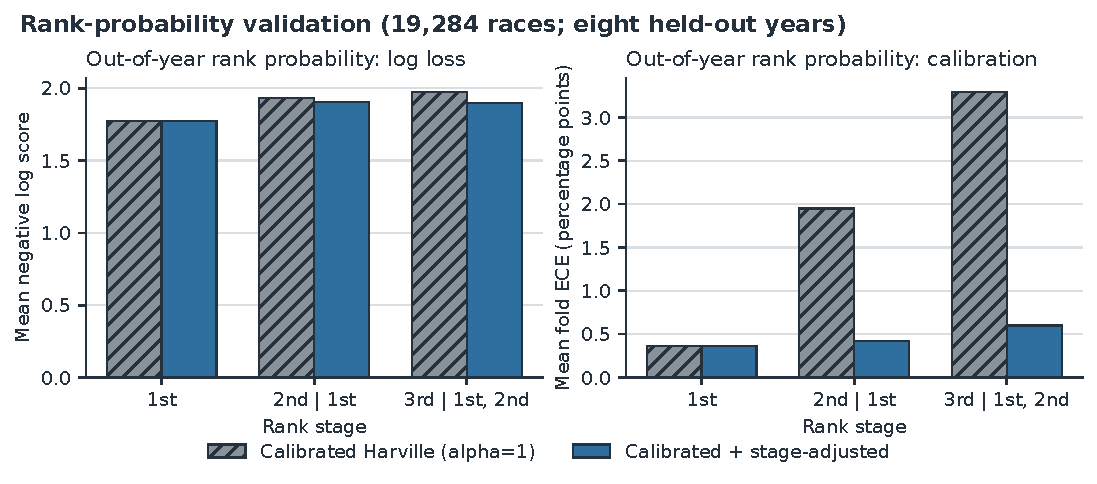
\includegraphics[width=0.96\textwidth]{figures/calibration-rank-probabilities.pdf}
\caption{조건부 순위확률의 연도 밖 로그손실과 보정오차}
\label{fig:behavioral-rank-validation}
\end{figure}

표~\ref{tab:behavioral-rank-validation}에서 1위 확률은 두 모형이 같고, 차이는
2·3위의 조건부 단계에서 생긴다. 단계조정 모형은 Harville 대비 2위 로그손실을
1.47\%, 3위 로그손실을 3.66\% 낮춘다. 평균 fold ECE도 2위에서
1.95에서 0.42 퍼센트포인트로, 3위에서 3.29에서 0.60 퍼센트포인트로
감소한다. 남은 선택집합이 10마리일 때 단계 온도계수는 여덟 fold에서 2위
0.729--0.746, 3위 0.565--0.579 범위다. 따라서 이하의 행동모형 비교는
실현 착순을 설명하지 못하는 임의의 Harville 입력이 아니라, 연도 밖에서
검증된 단계조정 순위확률을 선호 명세로 사용한다.

\subsection{순서형 가격벡터의 축약과 순차평가}

\begin{table}[htbp]
\centering
\caption{선호 명세의 행동가격모형 비교. 단계조정 순위확률과 Prelec
가중함수를 사용한다. 공통지지는 각 청구권의 모든 가중함수 인수가 훈련 단승확률의
1--99백분위 안에 드는 비율이다. M-U는 비모수적으로 회수하면 M-R과
관측적으로 같으므로 생략한다.}
\label{tab:behavioral-model-comparison}
\resizebox{0.88\textwidth}{!}{\begin{tabular}{llrrrr}
\toprule
시장 & 모형 & 경주수 & 중앙 TV & 중앙 로그 RMSE & 공통지지 \\
\midrule
쌍승 & M-R & 18,720 & 0.2534 & 1.0149 & 69.5\% \\
쌍승 & M-S2 & 18,720 & 0.1263 & 0.4548 & 98.0\% \\
\addlinespace
삼쌍승 & M-R & 3,323 & 0.3179 & 0.9778 & 38.1\% \\
삼쌍승 & M-S2 & 3,323 & 0.2075 & 0.5633 & 98.0\% \\
삼쌍승 & M-S3 & 3,323 & 0.1577 & 0.4728 & 98.9\% \\
\addlinespace
복승 & M-R & 19,286 & 0.1834 & 0.8097 & 81.4\% \\
복승 & M-S2 & 19,286 & 0.1300 & 0.4521 & 96.1\% \\
\addlinespace
삼복승 & M-R & 15,864 & 0.2775 & 1.0444 & 63.9\% \\
삼복승 & M-S2 & 15,864 & 0.2204 & 0.7217 & 74.8\% \\
삼복승 & M-S3 & 15,864 & 0.1545 & 0.5185 & 96.5\% \\
\bottomrule
\end{tabular}
}
\end{table}

\begin{figure}[htbp]
\centering
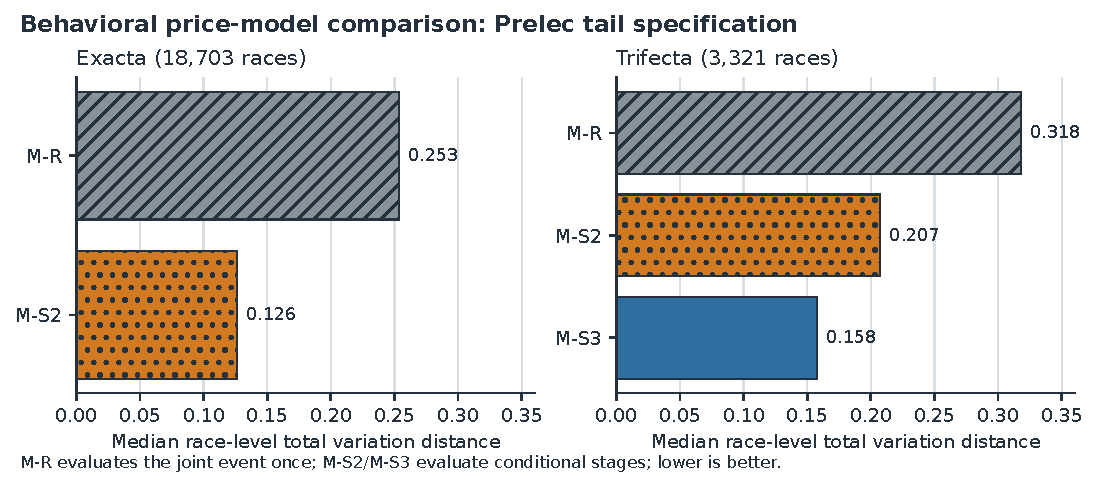
\includegraphics[width=0.96\textwidth]{figures/model-comparison-behavioral.pdf}
\caption{순서형 승식의 행동가격모형 TV 비교}
\label{fig:behavioral-ordered-comparison}
\end{figure}

쌍승에서 경주별 TV 중앙값은 M-R의 0.2534에서 M-S2의 0.1264로
낮아진다. 짝지은 개선폭 중앙값은 0.1230이고, 999회 경주일 군집
bootstrap 95\% 구간은 [0.1220, 0.1243]이다. 삼쌍승에서는 M-R
0.3178, M-S2 0.2075, M-S3 0.1578 순이다. M-R 대비 M-S3의
개선폭 중앙값은 0.1554[0.1533, 0.1577]이고, M-S2 대비 세 번째
단계를 분리했을 때에도 0.0498[0.0485, 0.0511]만큼 낮아진다.
이 네 비교의 연도별 TV 개선 중앙값은 모두 8개 연도에서 양수다.

이 결과가 하나의 손실함수에만 의존하는 것은 아니다. JS에서도 같은 순위를
얻고, 끝점 고정 isotonic 명세와 Prelec 명세의 TV 방향도 일치한다. 다만
삼쌍승 M-S3의 M-S2 대비 로그 RMSE 개선은 Prelec 명세에서 8개 연도 중
6개, isotonic 명세에서 5개 연도에서만 양수다. 따라서 세 번째 평가단계가
모든 손실함수와 모든 연도를 지배한다고 표현하지 않고, TV와 JS에서 일관된
우위라고 제한한다. power 명세에서는 순서형 M-R·M-S2·M-S3의 TV가
기계정밀도 수준에서 일치하여, 곱셈적 가중함수의 축약 불변성이 예상대로
재현된다.

\subsection{복승·삼복승의 무순서 외부검증}

\begin{figure}[htbp]
\centering
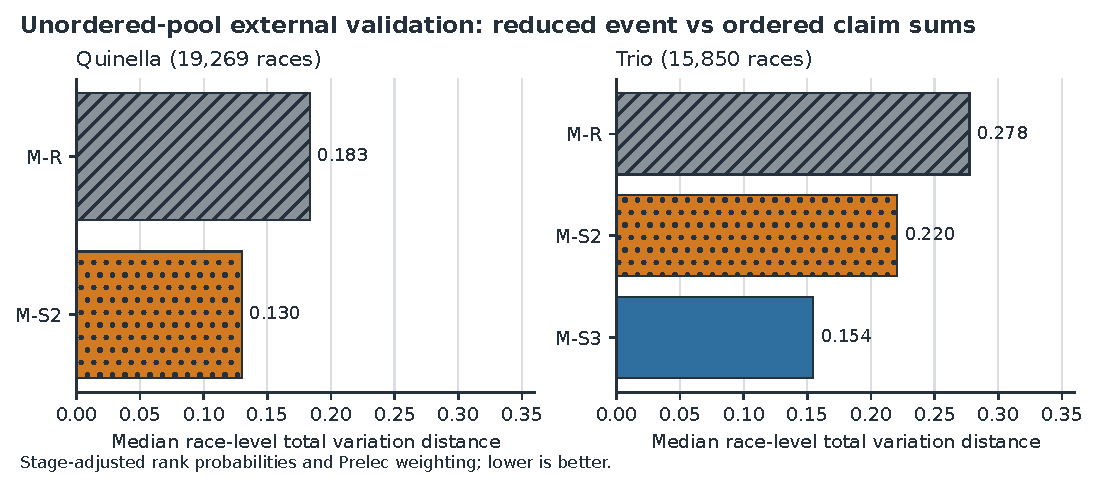
\includegraphics[width=0.96\textwidth]{figures/model-comparison-unordered.pdf}
\caption{무순서 승식의 외부검증: 결합사건의 축약평가와 순서형 청구권
예측가격 합의 비교}
\label{fig:behavioral-unordered-comparison}
\end{figure}

\begin{table}[htbp]
\centering
\caption{선호 명세의 짝지은 TV 개선폭. 구간은 경주일을 군집으로 999회
재표집한 개별 95\% bootstrap 구간이며 다중비교 보정을 적용하지 않았다.}
\label{tab:behavioral-model-improvements}
\resizebox{\textwidth}{!}{\begin{tabular}{lllrrr}
\toprule
시장 & 기준 & 비교모형 & TV 개선 중앙값 & 95\% 구간 & 양의 연도 \\
\midrule
쌍승 & M-R & M-S2 & 0.1230 & [0.1220, 0.1243] & 8/8 \\
\addlinespace
삼쌍승 & M-R & M-S2 & 0.1069 & [0.1049, 0.1082] & 8/8 \\
삼쌍승 & M-R & M-S3 & 0.1554 & [0.1533, 0.1577] & 8/8 \\
삼쌍승 & M-S2 & M-S3 & 0.0498 & [0.0485, 0.0511] & 8/8 \\
\addlinespace
복승 & M-R & M-S2 & 0.0557 & [0.0544, 0.0569] & 8/8 \\
\addlinespace
삼복승 & M-R & M-S2 & 0.0543 & [0.0538, 0.0548] & 8/8 \\
삼복승 & M-R & M-S3 & 0.1213 & [0.1201, 0.1228] & 8/8 \\
삼복승 & M-S2 & M-S3 & 0.0663 & [0.0654, 0.0675] & 8/8 \\
\bottomrule
\end{tabular}
}
\end{table}

순서 없는 풀에서도 같은 방향이 유지된다. 복승의 TV 중앙값은 결합확률합을
한 번 평가하는 M-R에서 0.1833이고, 두 쌍승 순서의 M-S2 청구권 가격을
합하면 0.1300이다. 짝지은 개선폭은 0.0557[0.0544, 0.0569]이며
8개 연도 모두 양수다. 삼복승은 M-R 0.2775, 여섯 삼쌍승 순서의 M-S2 합
0.2204, M-S3 합 0.1545 순이다. M-R 대비 M-S3 개선폭은
0.1213[0.1201, 0.1228], M-S2 대비 M-S3 개선폭은
0.0663[0.0654, 0.0675]이고 두 비교 모두 8개 연도에서 양수다.
복승·삼복승에서는 로그 RMSE와 JS도 같은 연도별 방향을 보인다.

이 검정은 무순서 승식에 자의적인 첫 번째 말을 지정한 결과가 아니다. M-R은
두 순서 또는 여섯 순서의 객관확률을 먼저 합한 뒤 $w$를 한 번 적용한다.
M-S2와 M-S3은 각 순서형 청구권의 단계별 점수를 계산한 뒤 그 청구권 가격을
합한다. 따라서 순서형 풀에서 식별한 비축약 표현이 별도 무순서 풀의 전체
가격벡터로 이동하는지를 묻는 진정한 leave-one-pool-out 외부검증이다.

\subsection{과거 자료만 사용하는 시간순 검증}

연도 제외 교차적합은 검증연도보다 뒤의 자료도 훈련에 사용할 수 있다. 이를
배제하기 위해 2017년부터 각 검증연도 직전까지의 자료만 누적하여 같은 모형을
다시 추정했다. 2016년은 이전 훈련연도가 없으므로 시간순 검증에서 제외한다.
이 expanding-window 표본은 착순확률 17,745개 경주, 쌍승 17,324개,
삼쌍승 3,130개, 복승 17,736개와 삼복승 14,840개 비검열 경주를 포함한다.

시간순 검증에서도 단계조정 모형의 로그손실은 Harville 대비 2위에서 1.47\%,
3위에서 3.65\% 낮다. 이는 앞서 보고한 19,284개 경주의 연도제외 3.66\%와
달리, 17,745개 경주의 과거연도 전용 표본에서 얻은 별도 추정치다. 선호 명세의
TV 중앙값은 쌍승에서 M-R 0.2664와
M-S2 0.1326, 삼쌍승에서 M-R 0.3258, M-S2 0.2143과 M-S3
0.1596이다. 복승은 0.1955와 0.1341, 삼복승은 0.2906, 0.2317과
0.1599 순이다. 표~\ref{tab:behavioral-time-forward}의 여덟 TV 대비는
모두 7개 시간순 검증연도에서 같은 방향을 유지한다.

\begin{table}[htbp]
\centering
\caption{과거 연도만 훈련에 사용한 시간순 검증의 짝지은 TV 개선폭. 구간은
경주일을 군집으로 999회 재표집한 개별 95\% bootstrap 구간이며 다중비교
보정을 적용하지 않았다.}
\label{tab:behavioral-time-forward}
\resizebox{\textwidth}{!}{\begin{tabular}{lllrrr}
\toprule
시장 & 기준 & 비교모형 & TV 개선 중앙값 & 95\% 구간 & 양의 연도 \\
\midrule
쌍승 & M-R & M-S2 & 0.1305 & [0.1291, 0.1318] & 7/7 \\
\addlinespace
삼쌍승 & M-R & M-S2 & 0.1073 & [0.1057, 0.1087] & 7/7 \\
삼쌍승 & M-R & M-S3 & 0.1615 & [0.1590, 0.1635] & 7/7 \\
삼쌍승 & M-S2 & M-S3 & 0.0534 & [0.0523, 0.0548] & 7/7 \\
\addlinespace
복승 & M-R & M-S2 & 0.0656 & [0.0642, 0.0672] & 7/7 \\
\addlinespace
삼복승 & M-R & M-S2 & 0.0559 & [0.0555, 0.0564] & 7/7 \\
삼복승 & M-R & M-S3 & 0.1294 & [0.1278, 0.1307] & 7/7 \\
삼복승 & M-S2 & M-S3 & 0.0721 & [0.0711, 0.0730] & 7/7 \\
\bottomrule
\end{tabular}
}
\end{table}

\subsection{공통지지와 식별의 한계}

\begin{figure}[htbp]
\centering
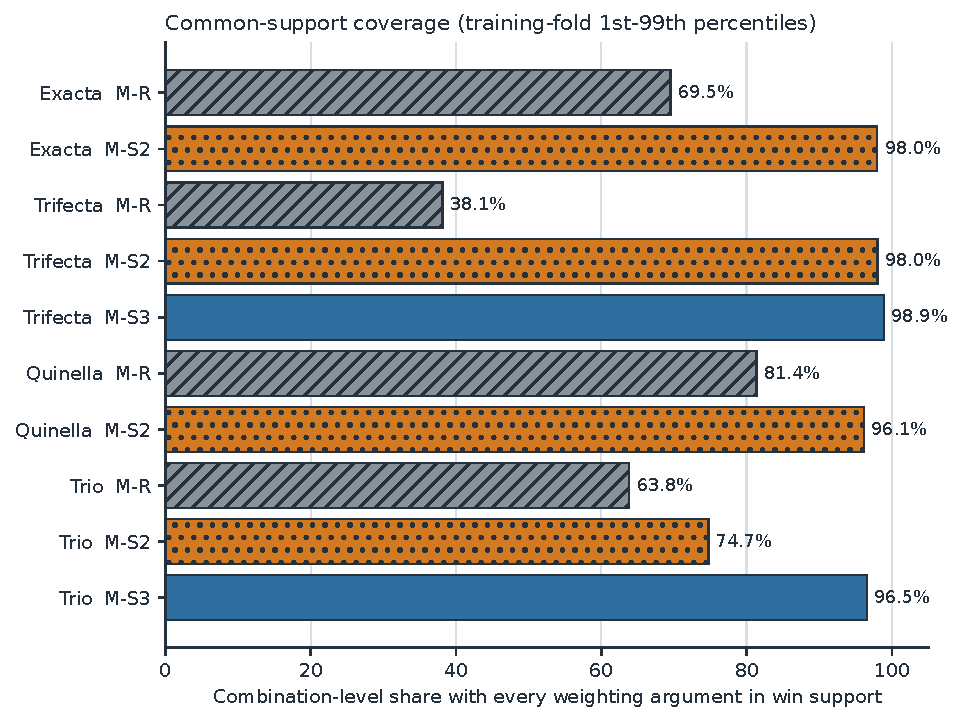
\includegraphics[width=0.92\textwidth]{figures/model-comparison-support.pdf}
\caption{훈련 단승확률 공통지지에 포함되는 가중함수 인수의 비율}
\label{fig:behavioral-support}
\end{figure}

% Source: outputs/behavioral_model_comparison.csv,
% probability_model=stage_temperature, tail_model=prelec, price_model=M-R,
% columns mean_support_share and all_arguments_supported_race_share.
M-R의 평균 공통지지는 쌍승 69.5\%, 삼쌍승 38.1\%, 복승 81.4\%,
삼복승 63.9\%다. M-S2는 각각 98.0\%, 98.0\%, 96.1\%, 74.7\%이고,
M-S3은 삼쌍승 98.9\%, 삼복승 96.5\%다. 더 엄격하게 한 경주의 모든 조합이
공통지지 안에 있는지를 보면 M-R의 비율은 쌍승 3.4\%, 삼쌍승 0.09\%,
복승 13.2\%, 삼복승 1.5\%에 그친다. 특히 희박한 결합확률을 한 번에
평가하는 M-R의 절대오차는 단승에서 관찰하지 못한 꼬리 외삽에 더 민감하다.
그러므로 선호 Prelec 명세의 절대 TV만으로 모형을 선택하지 않고, 공통지지를
명시한 isotonic 끝점 명세의 같은 방향과 power 음성대조를 함께 판정한다.

종합하면, 결과는 순서형·무순서형 네 승식 모두에서 복합사건의 완전 축약보다
조건부 순위단계를 분리한 가격표현과 더 잘 양립한다. 삼쌍승과 삼복승에서는
세 번째 단계를 별도로 평가한 M-S3이 TV 기준으로 추가 설명력을 갖는다.
그러나 M-U와 M-R은 단승 가격만으로 관측적으로 동등하고, 풀별 참가자 구성과
유동성도 관찰되지 않는다. 따라서 이 결과를 대표적 가격함수의 안정적인
비축약 표현에 대한 증거로 해석하되, 모든 개인의 확률오인이나 특정 인지과정을
직접 식별한 결과로 확대하지 않는다.

\section{결론}

이 논문은 같은 경주에 열린 여러 패리뮤추얼 시장을 하나의 순위 상태공간 위에
놓는다. 삼쌍승식은 상위 3마리의 순서를 구분하는 가장 세분된 청구권이며, 다른
주요 승식은 그 상태들을 합한 사건에 지급한다. 따라서 승식별 가격의 관계를
단순한 상관관계가 아니라 명시적인 가산 제약으로 검정할 수 있다.

이 설계가 제공하는 핵심 구분은 내부 일관성과 외부 정확도의 분리다. 삼쌍승식
가격이 단순 승식 가격을 잘 재구성한다면 여러 풀이 공통된 순위 구조를 반영한다는
증거가 된다. 그러나 그것만으로 그 구조가 객관적 확률과 일치한다고 말할 수는
없다. 실현 착순에 대한 예측력과 전통적인 인기마--비인기마 편향은 별도 검정으로
확인해야 한다. 이 구분을 유지하면 경마시장을 단순한 이상현상의 사례가 아니라,
서로 다른 차원의 시장이 정보를 집계하고 전달하는 방식을 관찰할 수 있는
실험장으로 사용할 수 있다.


\bibliographystyle{apalike}
\bibliography{references}

\end{document}
